\documentclass{article}
\usepackage{amsmath, amssymb, kotex, hyperref, graphicx, mdframed, setspace,enumitem}
\usepackage[a4paper, margin = 40pt]{geometry}
\setstretch{1.5}
\begin{document}
\title{시계열 회귀분석(Time Series Regression - 3)}
\author{강의 : 김성범 교수님\\ 정리 :  김선중}
\date{\today}
\maketitle

이것은 \href{https://youtu.be/5QnR4L3KGz4}{Time Series Regression - Part 3} 강의에 대한 노트이다.
\tableofcontents

\bigskip\bigskip
%\newpage
아래 식에서 보듯이, 많은 경우에 시계열은 추세(trend)와 계절성(seasonality), 그리고 오차로 이루어져있다.
이번 강의에서는 seaonsal variation을 모델링하는 네 가지 모델에 대해서 다루는 것 같다.
그것들은
\begin{itemize}[itemsep=0pt,parsep=0pt]
\item
binary variable models
\item
trigonometric models
\item
growth curve models
\item
first-order autoregressive process
\end{itemize}
이다.
이 중에서 앞의 세 개는 고전적인 방법이고 마지막 방법이 앞으로 계속 사용할 방법인 것 같다.

\begin{center}
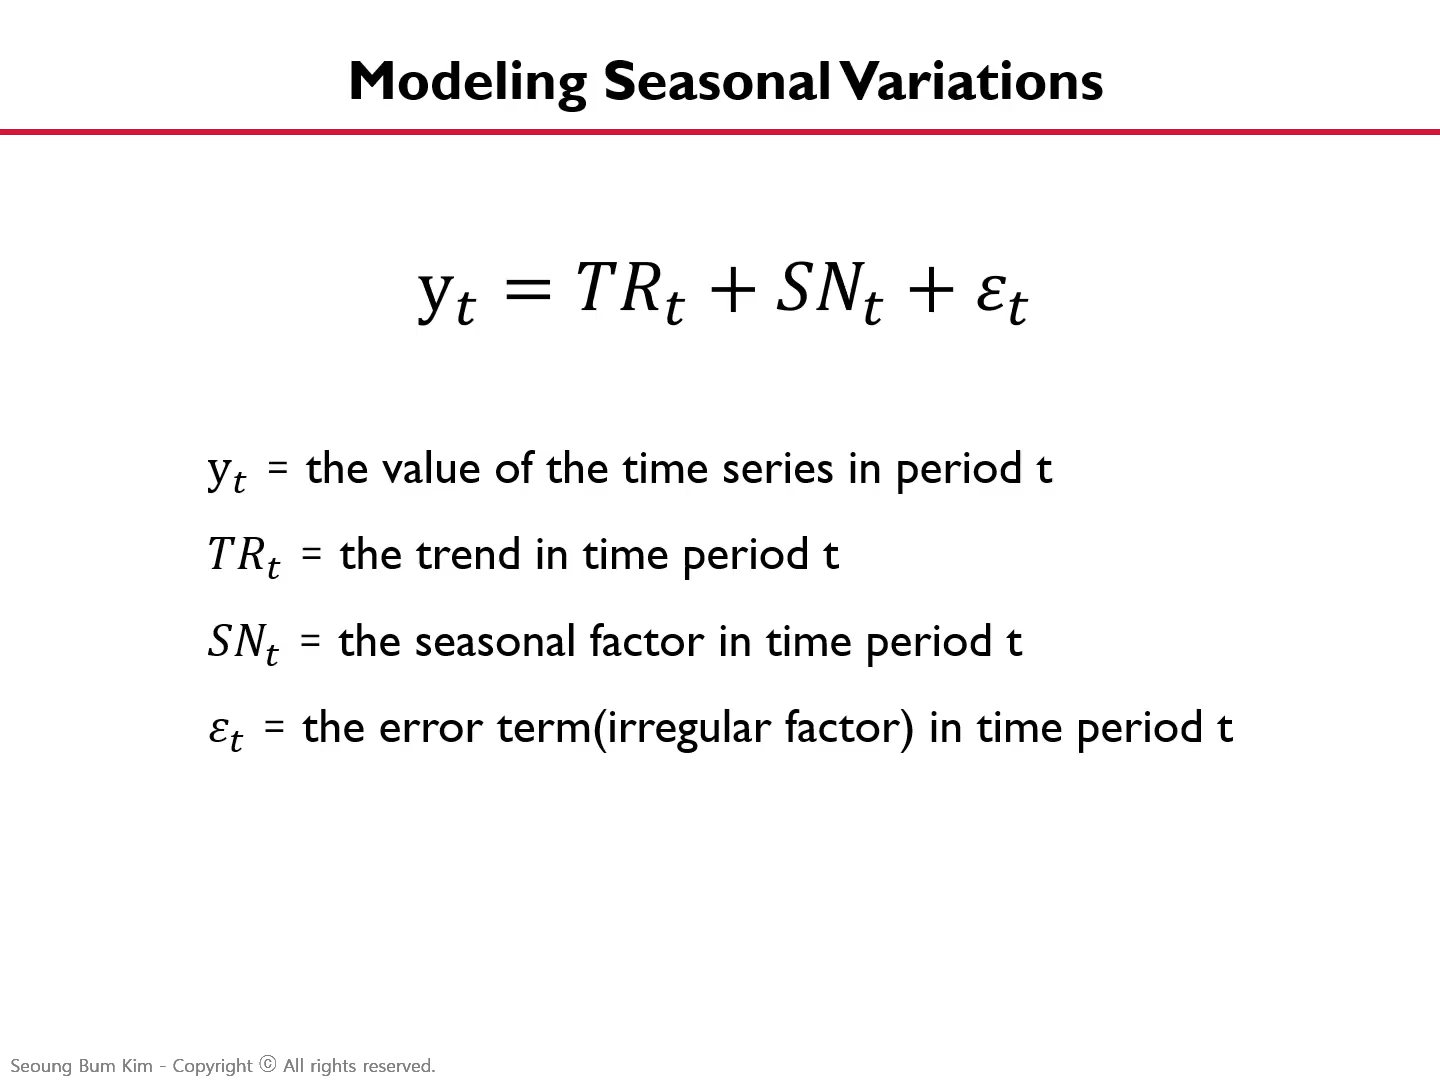
\includegraphics[width=.5\textwidth]{model_0}
\end{center}

이번 정리부터는 유튜브 캡쳐를 나열한 후 정리하려고 하고, 너무 많은 내용을 적기보다는 강의 내용 자체에만 충실하게 적어보려고 한다.

%%
\section{Binary Variable Models}
\begin{center}
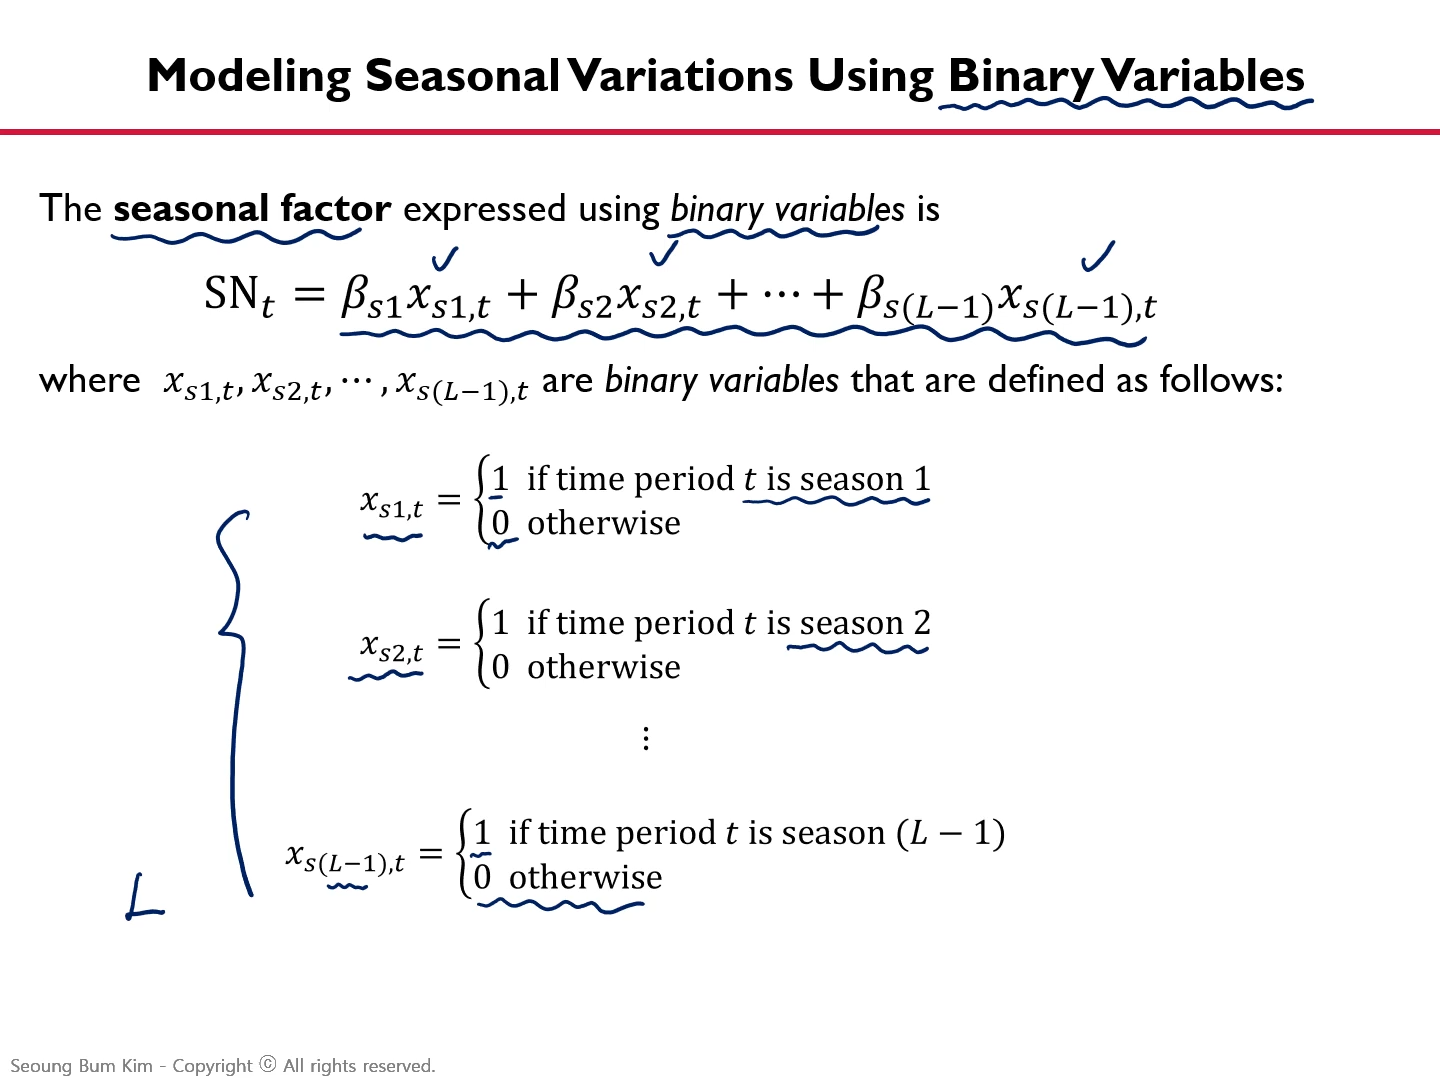
\includegraphics[width=.45\textwidth]{model_1-1}
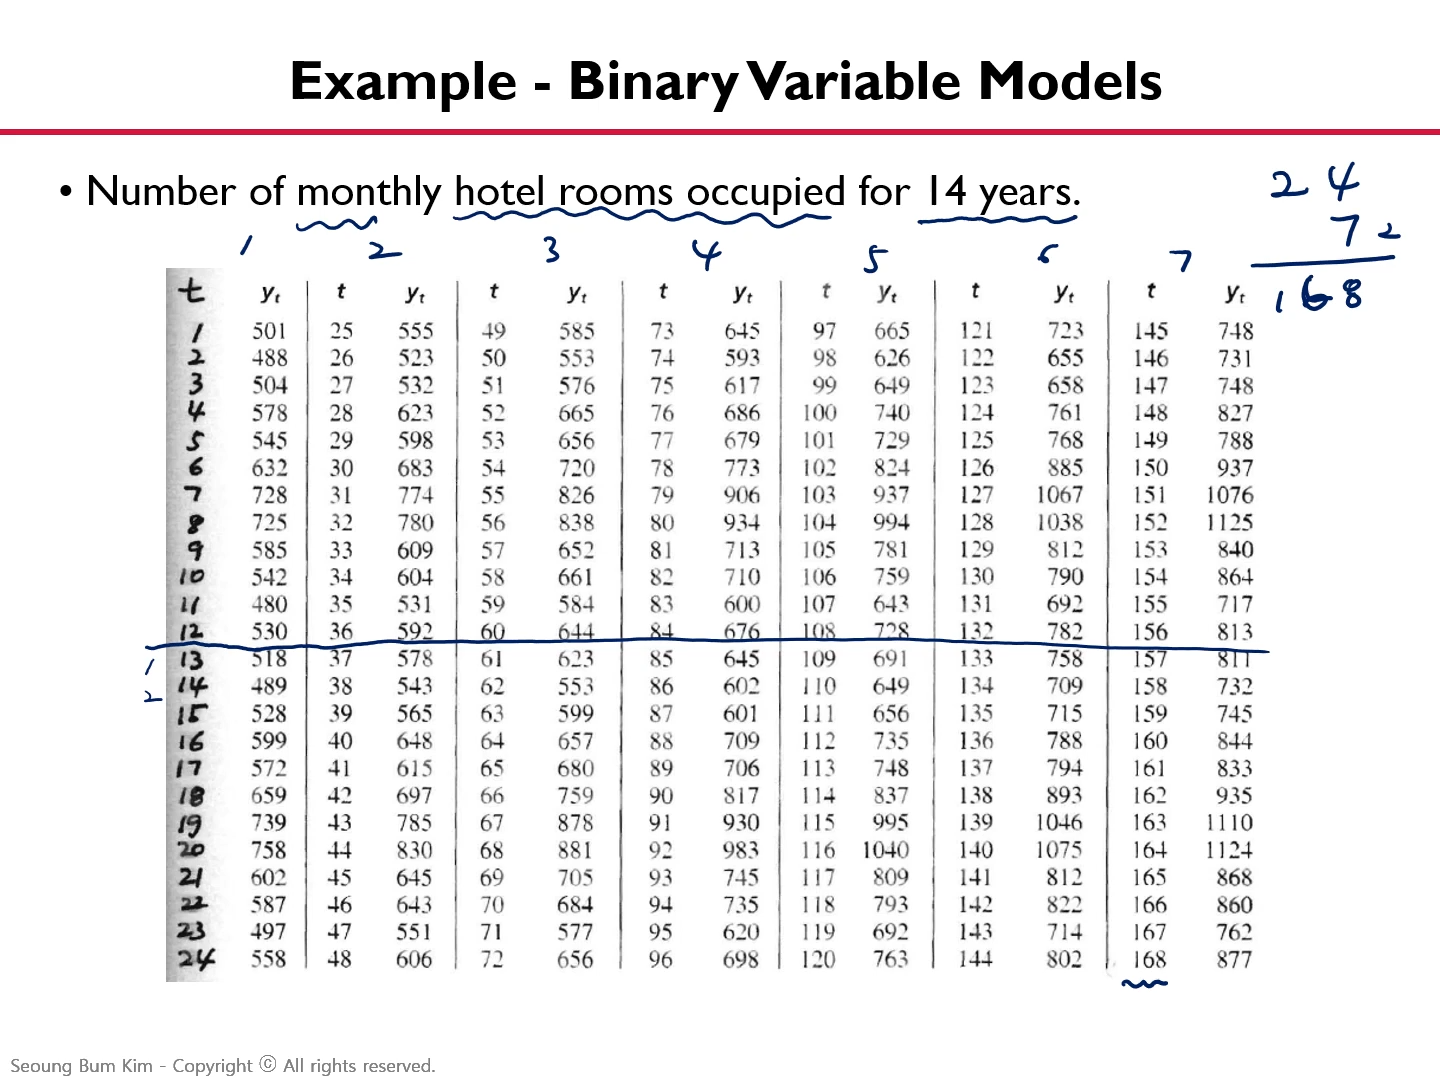
\includegraphics[width=.45\textwidth]{model_1-2}
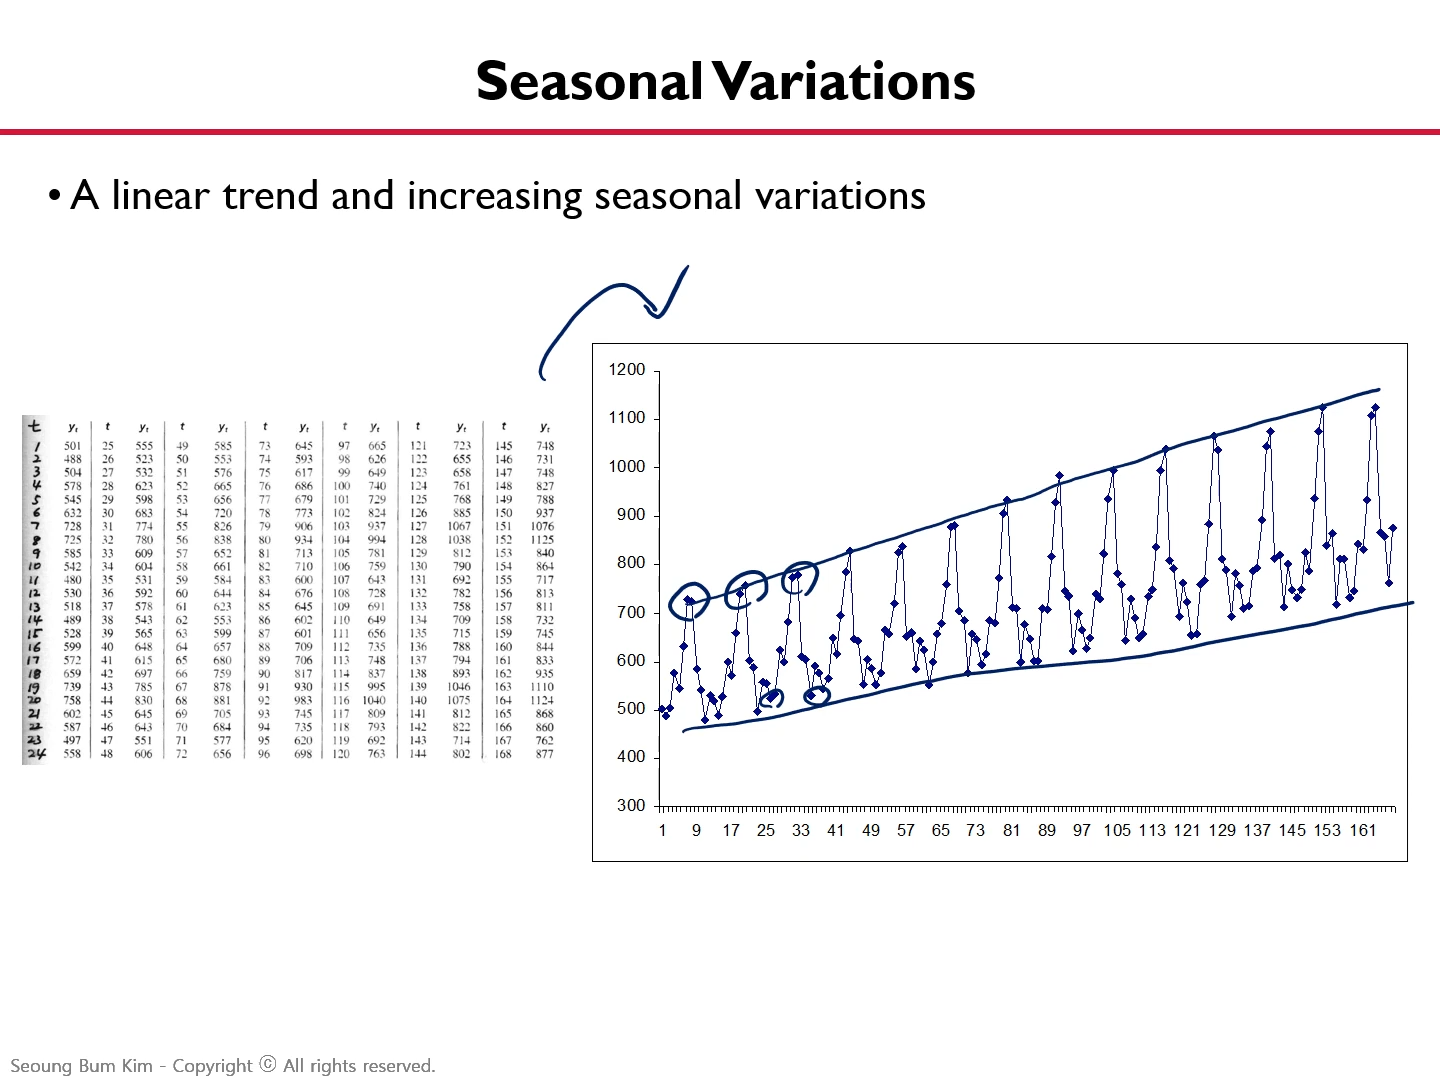
\includegraphics[width=.45\textwidth]{model_1-3}
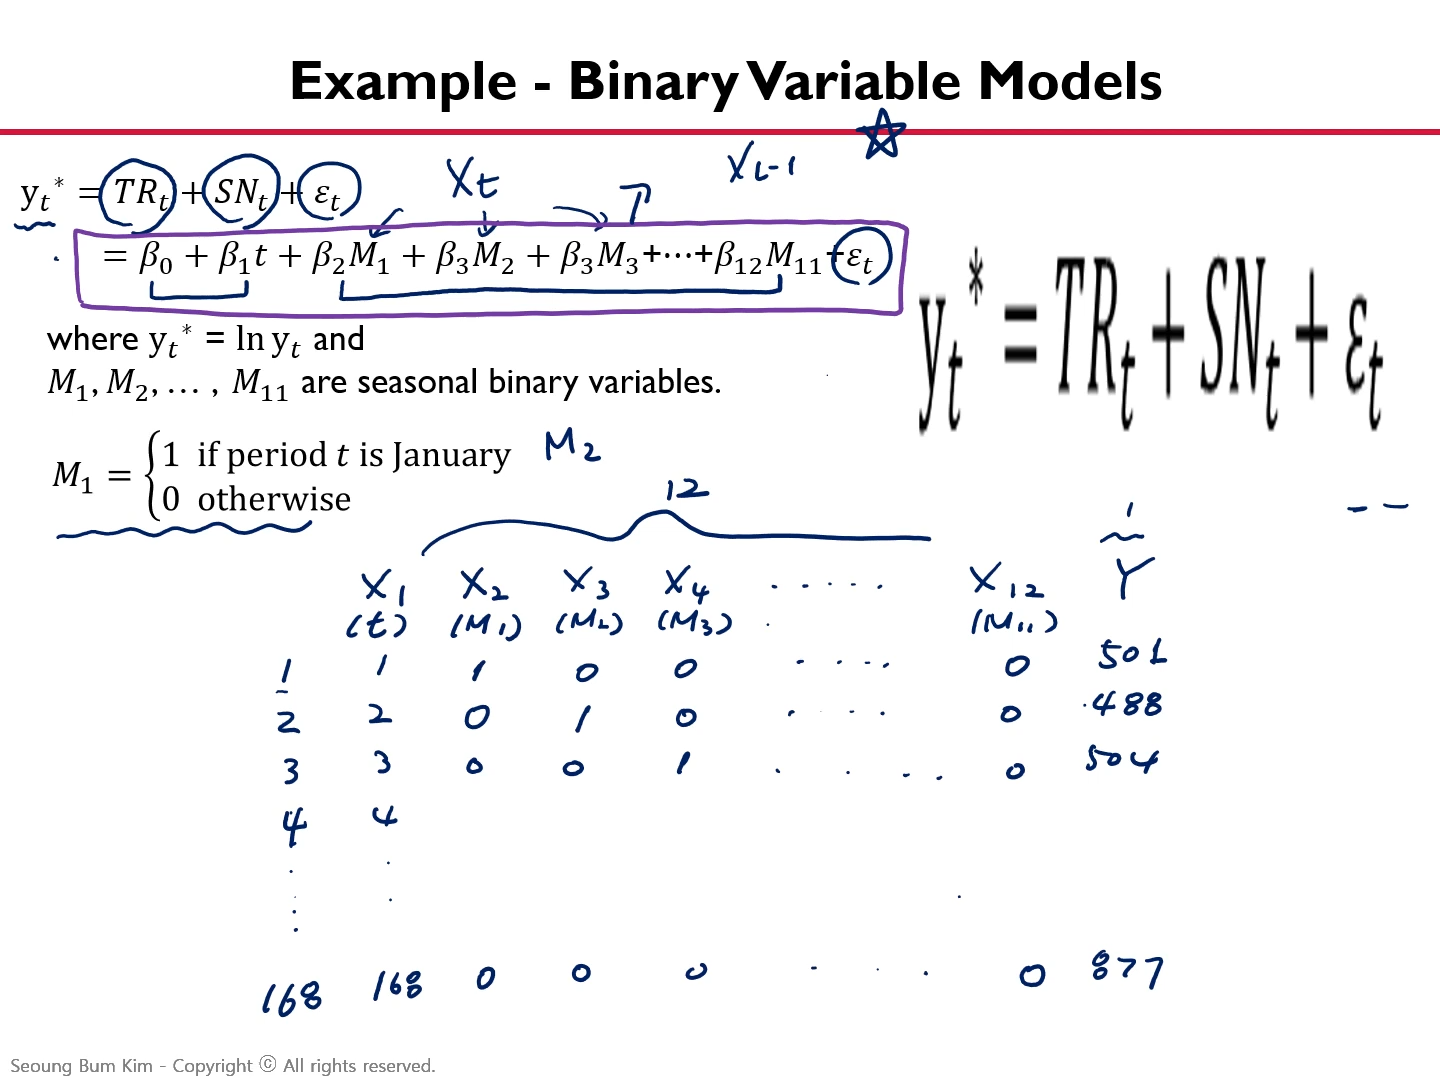
\includegraphics[width=.45\textwidth]{model_1-4}
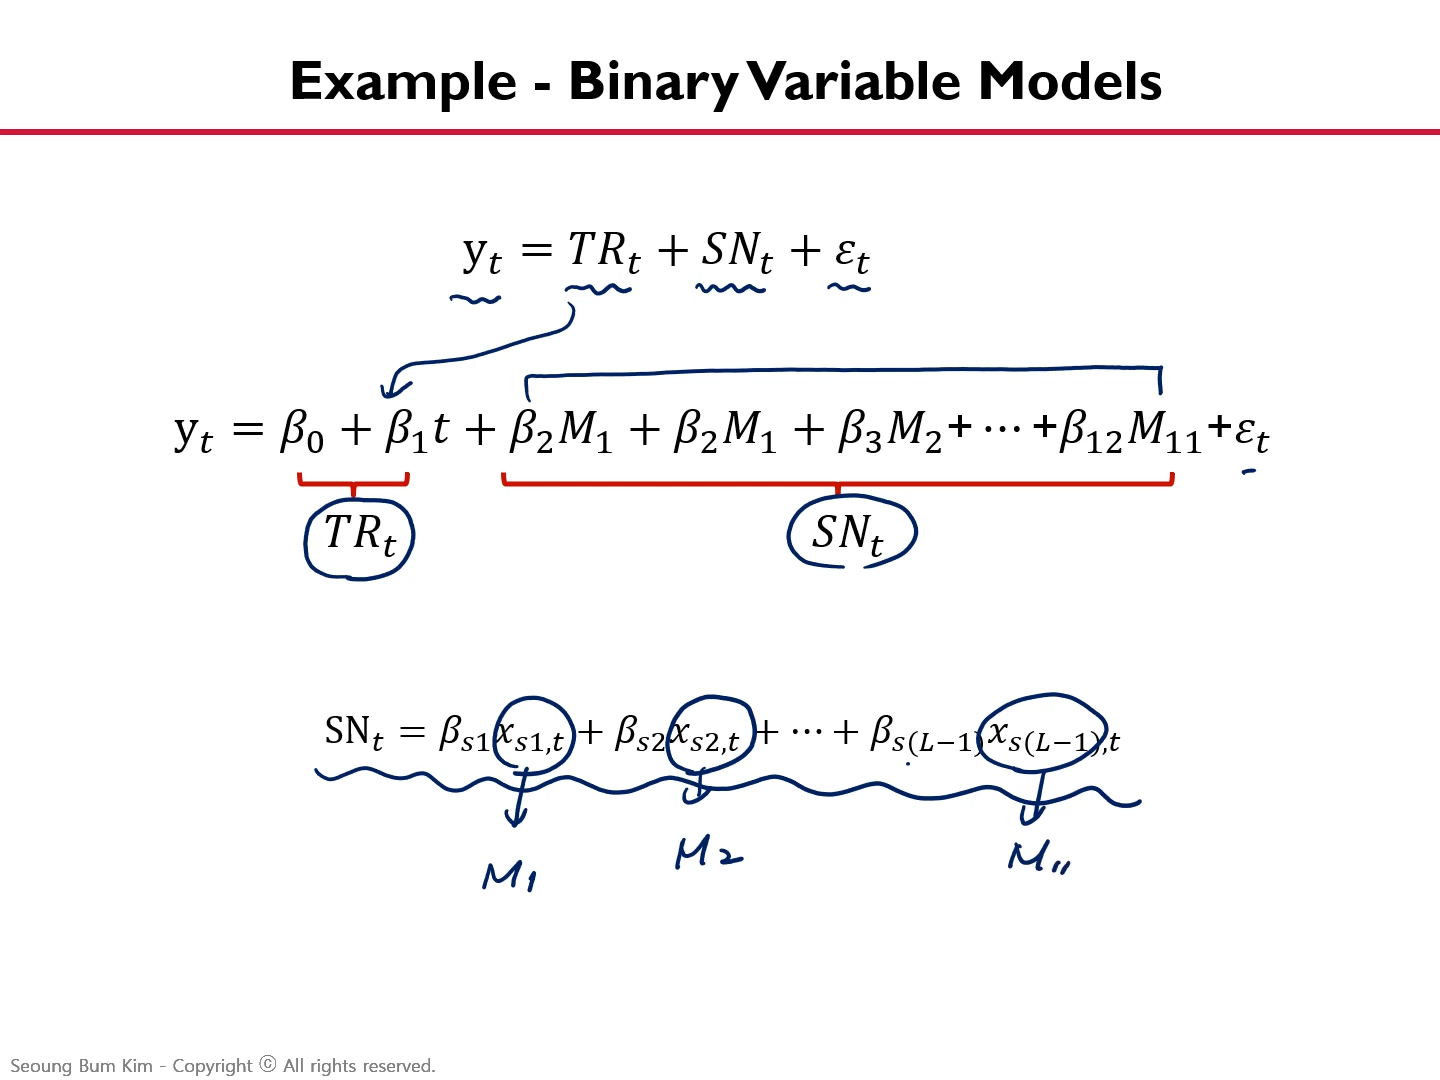
\includegraphics[width=.45\textwidth]{model_1-5}
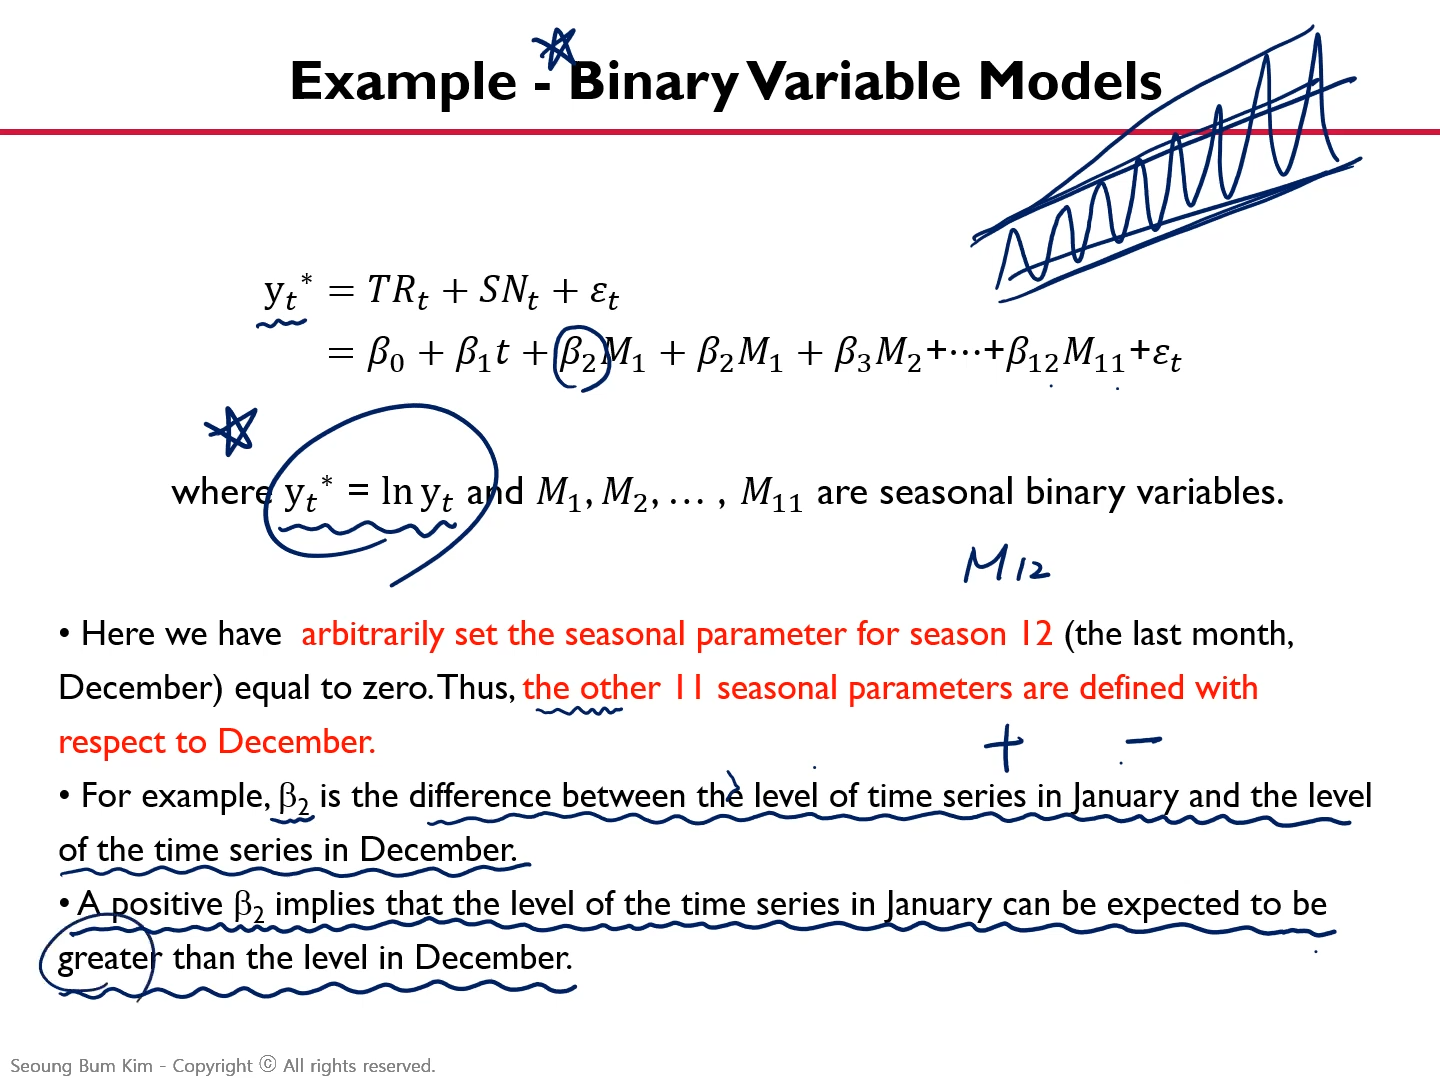
\includegraphics[width=.45\textwidth]{model_1-6}
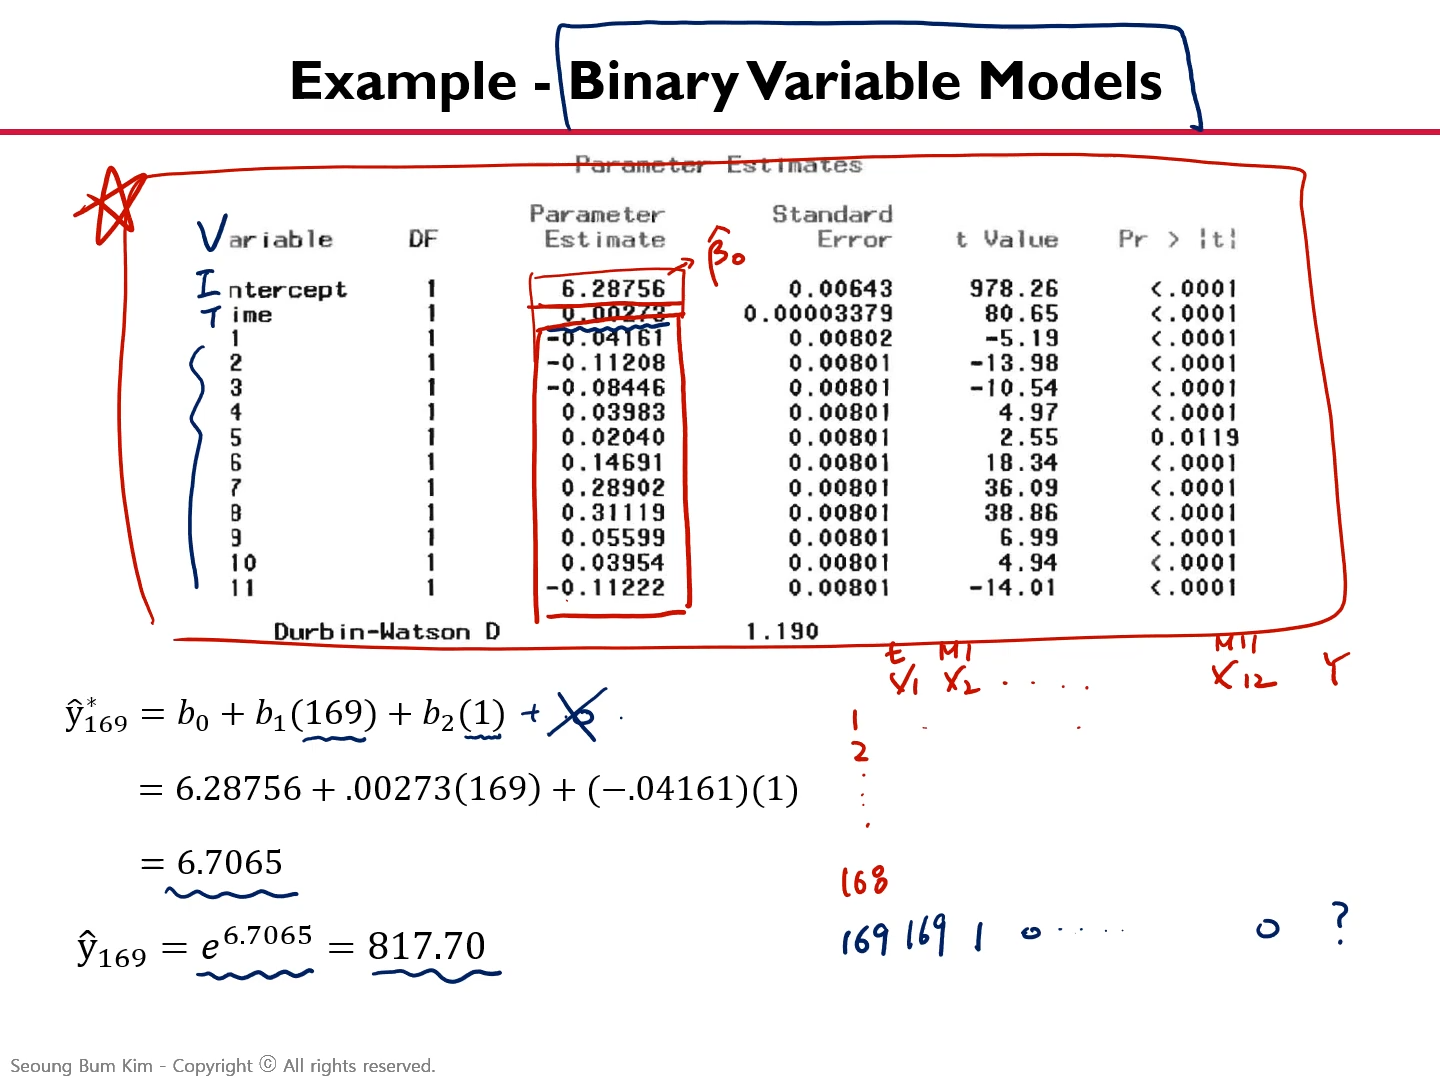
\includegraphics[width=.45\textwidth]{model_1-7}
\end{center}

seasonal variation을 다루기 위한 여러 모델들 중 첫번째로 다루는 모델은 binary variable model이다.
예시로 주어지고 있는 데이터셋은 한 호텔의 투숙된 객실 수에 대한 데이터이다.
시간 \(t\)의 단위는 `월'로 주어져있고, 총 7년의 데이터가 있으므로 \(t\in\{1, 2,\cdots,168\}\)이다.
종속변수는 \(y\)이고 독립변수는 \(x\)이지만, \(x_t=t\)라는 점에서 독립변수를 그냥 \(t\)라고 봐도 될 것 같다.
다시 말해서, 몇 번째 달(\(t\))에 몇 개의 객실들(\(y\))이 투숙되어 있는지 하는 단변수 회귀 (univariate regression) 문제이다.

이전 강의의 예에서는 추세(trend, $TR_t$)만을 예측모델로 잡았었다. 하지만, 세 번째 슬라이드에서 보듯 계절성이 뚜렷이 드러나고 있으므로, 예측모델 \(f_\beta\)을 설정할 때 추세 말고도 계절성(seasonal variation, $SN_t$)도 고려할 것이다.
즉
\begin{equation}\label{model_1-1}
f_\beta(t) = TR_t+SN_t
\end{equation}
이고
\[y_t=f_\beta(t)+\epsilon_t\]
이다.
추세는 일차함수(affine function)로 표현할 것이어서
\[TR_t = \beta_0+\beta_1 t\]
이고, 계절성은 각각의 계절에 대하여 상수회귀(no trend, constant regression)로 둔다.
식으로 표현하면
\[SN_t = \begin{cases}
\beta_2&(t=12n+1)\\
\beta_3&(t=12n+2)\\
&\vdots\\
\beta_{12}&(t=12n+11)\\
0&(t=12n+12)\\
\end{cases}\qquad\qquad(\text{단, \(n=0,1,2,\cdots,6)\)}\]
이다.
이것을 표현하기 위해서 강의에서는 \(M_1\), \(M_2\), \(\cdots\), \(M_{11}\)을 사용하고 있는데, 이건 각 월에 대한 characteristic function (indicator function)으로 이해하면 될 것 같다.
여하튼, 식 \eqref{model_1-1}을 다시 정리하면
\begin{equation}\label{model_1-2}
f_\beta(t) = \begin{cases}
\beta_0+\beta_2+\beta_1t&(t=12n+1)\\
\beta_0+\beta_3+\beta_1t&(t=12n+2)\\
&\vdots\\
\beta_0+\beta_{12}+\beta_1t&(t=12n+11)\\
\beta_0+\beta_1t&(t=12n+12)\\
\end{cases}\qquad\qquad(\text{단, \(n=0,1,2,\cdots,6)\)}
\end{equation}
이 된다.
%\(M_{12}\)는 굳이 사용하지 않았다.
각 월(1월 \(\sim\) 11월)에 대한 정보를 담고 있는 항은 \(\beta_2\), \(\cdots\), \(\beta_{12}\)이다.
그리고 12월에 대한 정보를 담고 있는 항은 없다.
하지만 문제가 되지 않는다.

다시 말해서, 1월부터 11월까지의 월들에 각각 어떤 기본값을 부여할 지에 대해서는 매개변수 \(\beta_2\), \(\cdots\), \(\beta_{11}\)로 조정하면 된다.
하지만, \(y\)절편에 해당하는 \(\beta_0\)를 이미 설정해놓았으므로, 12월에는 \(\beta_0\)라는 기본값을 부여받게 되는 것이다.
12월에 대한 정보는 \(\beta_0\)를 통해 조정될 수 있는 것이다.
새로운 매개변수 \(\beta_{12}\)를 도입할 수도 있지만, 굳이 그렇게 하는 게 의미가 없는 것이다.

그런데, 어차피 그렇게 할거면, trend를 설정할 때, \(y\)절편이 없는 일차함수로 잡은 다음 \(M_1\), \(M_2\), \(\cdots\), \(M_{12}\)를 설정해도 같은 의미가 될 것이다.
그렇게 하는 편이 보기에 깔끔해보인다.
그러니까
\[SN_t = \begin{cases}
\beta_1&(t=12n+1)\\
\beta_2&(t=12n+2)\\
&\vdots\\
\beta_{12}&(t=12n+12)
\end{cases}\qquad\qquad(\text{단, \(n=0,1,2,\cdots,6)\)}\]
로 두고
\[f_\beta(t) = \begin{cases}
\beta_0t+\beta_1&(t=12n+1)\\
\beta_0t+\beta_2&(t=12n+2)\\
&\vdots\\
\beta_0t+\beta_{12}&(t=12n+12)
\end{cases}\qquad\qquad(\text{단, \(n=0,1,2,\cdots,6)\)}\]
로 두는 것이 더 깔끔하면서도, 기존 방법과 완전히 같은 방법이지 않을까 한다.
하지만, 아마도 기존 방법이 통계 방면에서의 관습인 게 아닐까 싶기도 하다.

이렇게 parametric model \(f_\beta\)를 설정했다.
그 다음으로 하는 것은 기존의 회귀분석(ordinary regression analysis)을 진행하는 것이다.
강의에서는 45분 32초쯤에 `일반적인 최소제곱법(LSE, least square estimation ; OLS ordinary least square, ordinary least squares)'을 사용하는 것이다.
표에서 관측치가 주어져있었다.
\begin{equation}\label{observations}
\begin{aligned}
\text{관측치}
&=\{(t,y_t):t=1,2,\cdots,168\}\\
&=\{(1,501), (2,488),\cdots,(168,877)\}
\end{aligned}
\end{equation}
이걸 가지고 MSE를 계산하면
\begin{equation}\label{MSE}
\text{MSE}=\frac1{168}\sum_{t=1}^{168}\left(y_t-f_\beta(t)\right)^2
\end{equation}
이 된다.
\(MSE\)를 \(\beta_0\), \(\beta_1\), \(\cdots\), \(\beta_{11}\)로 편미분한 것을 0으로 두면 미지수가 12개이고 식이 12개인 연립방정식이 나오는데, 그 연립방정식을 풀어 근을 \(\beta_0=\hat\beta_0\), \(\beta_1=\hat\beta_1\), \(\cdots\), \(\beta_{11}=\hat\beta_{11}\) 들을 가지고 최적의 함수 \(\hat f\)를 찾을 수 있다.

이 계산들은 보통은 컴퓨터를 통해, 몇개의 명령어를 입력하여 계산하는 것 같고, 마지막 캡쳐의 표에 이 \(\hat\beta_i\)들의 값이 적혀있는 것으로 보인다.

%%
\section{Trigonometric Models}
\begin{center}
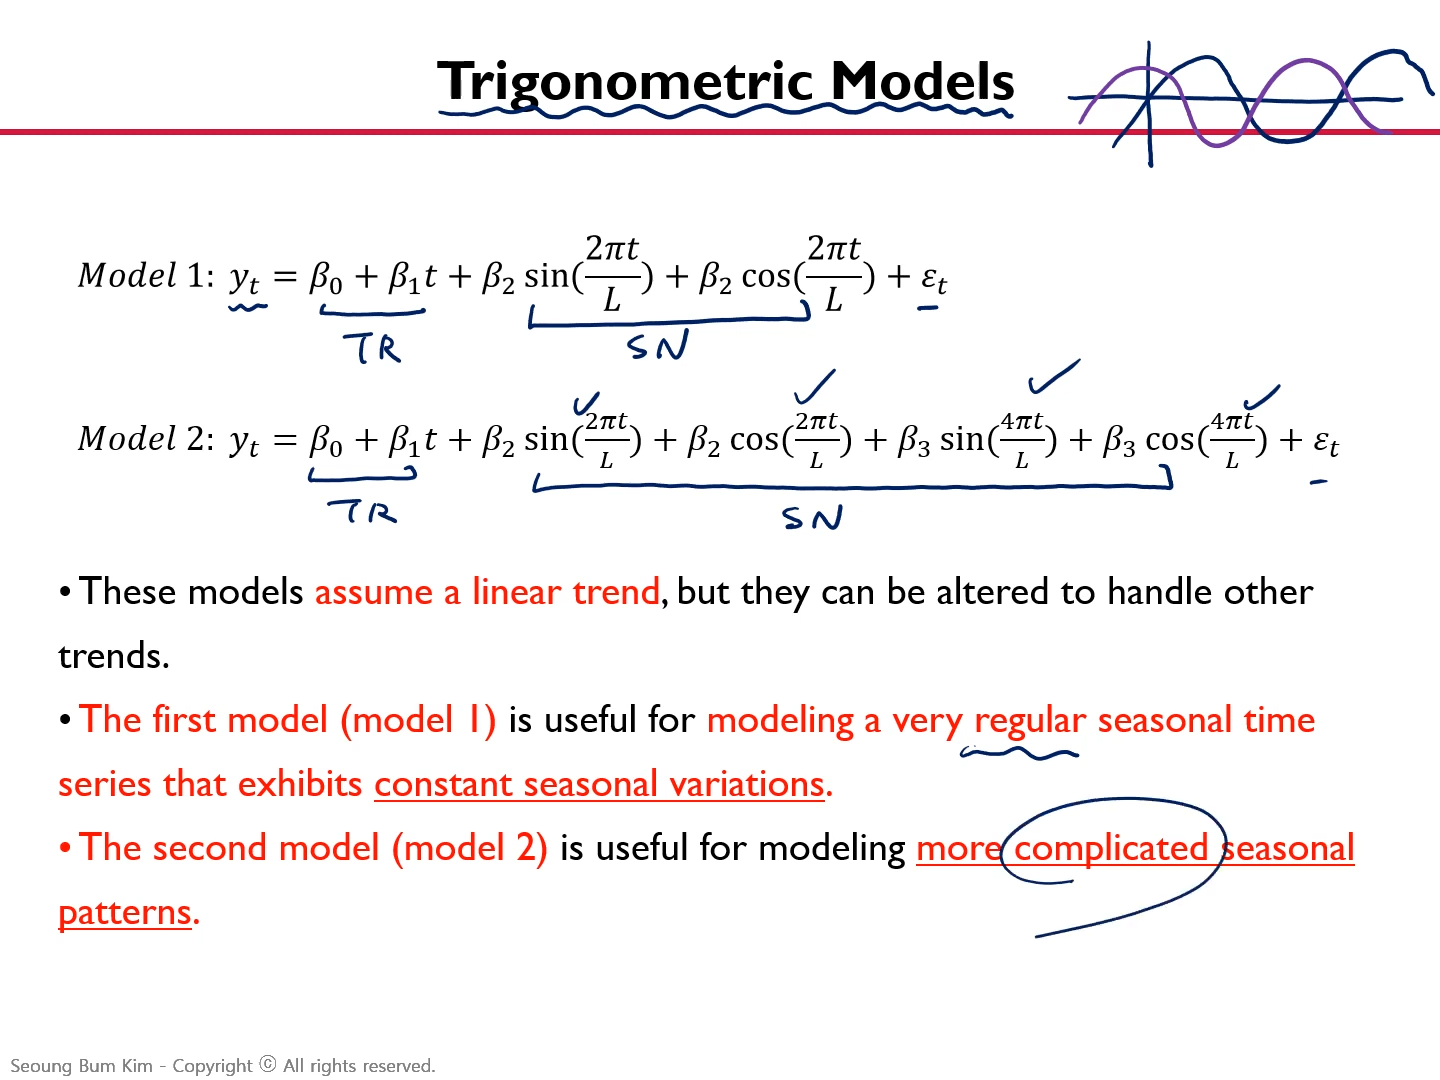
\includegraphics[width=.45\textwidth]{model_2-1}
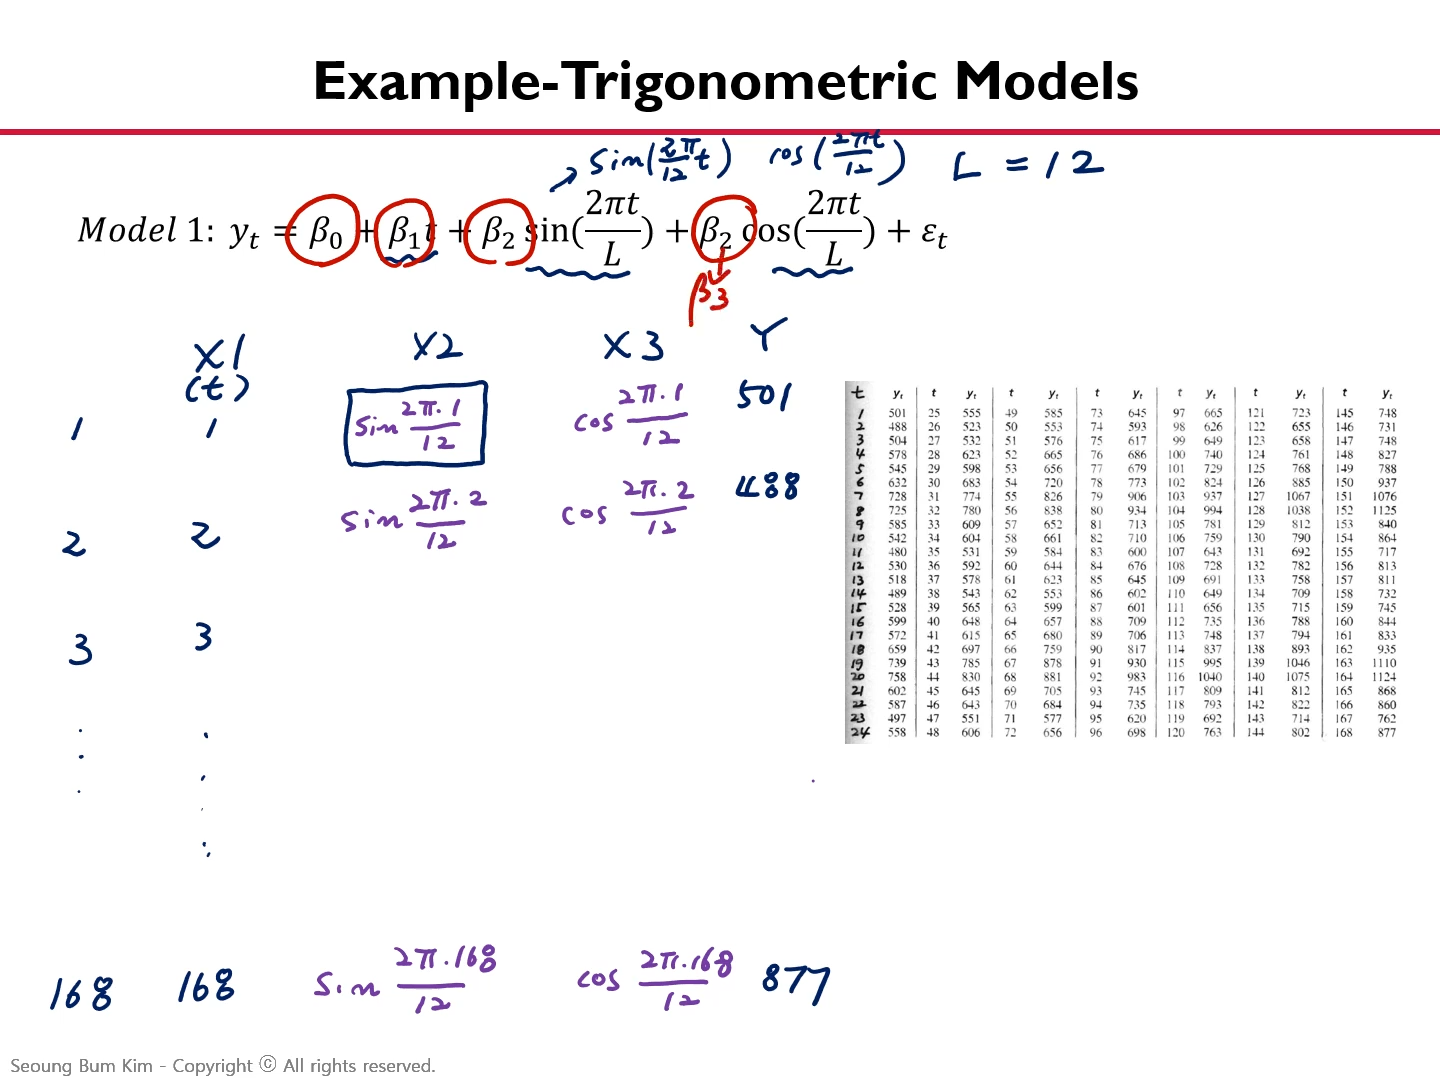
\includegraphics[width=.45\textwidth]{model_2-2}
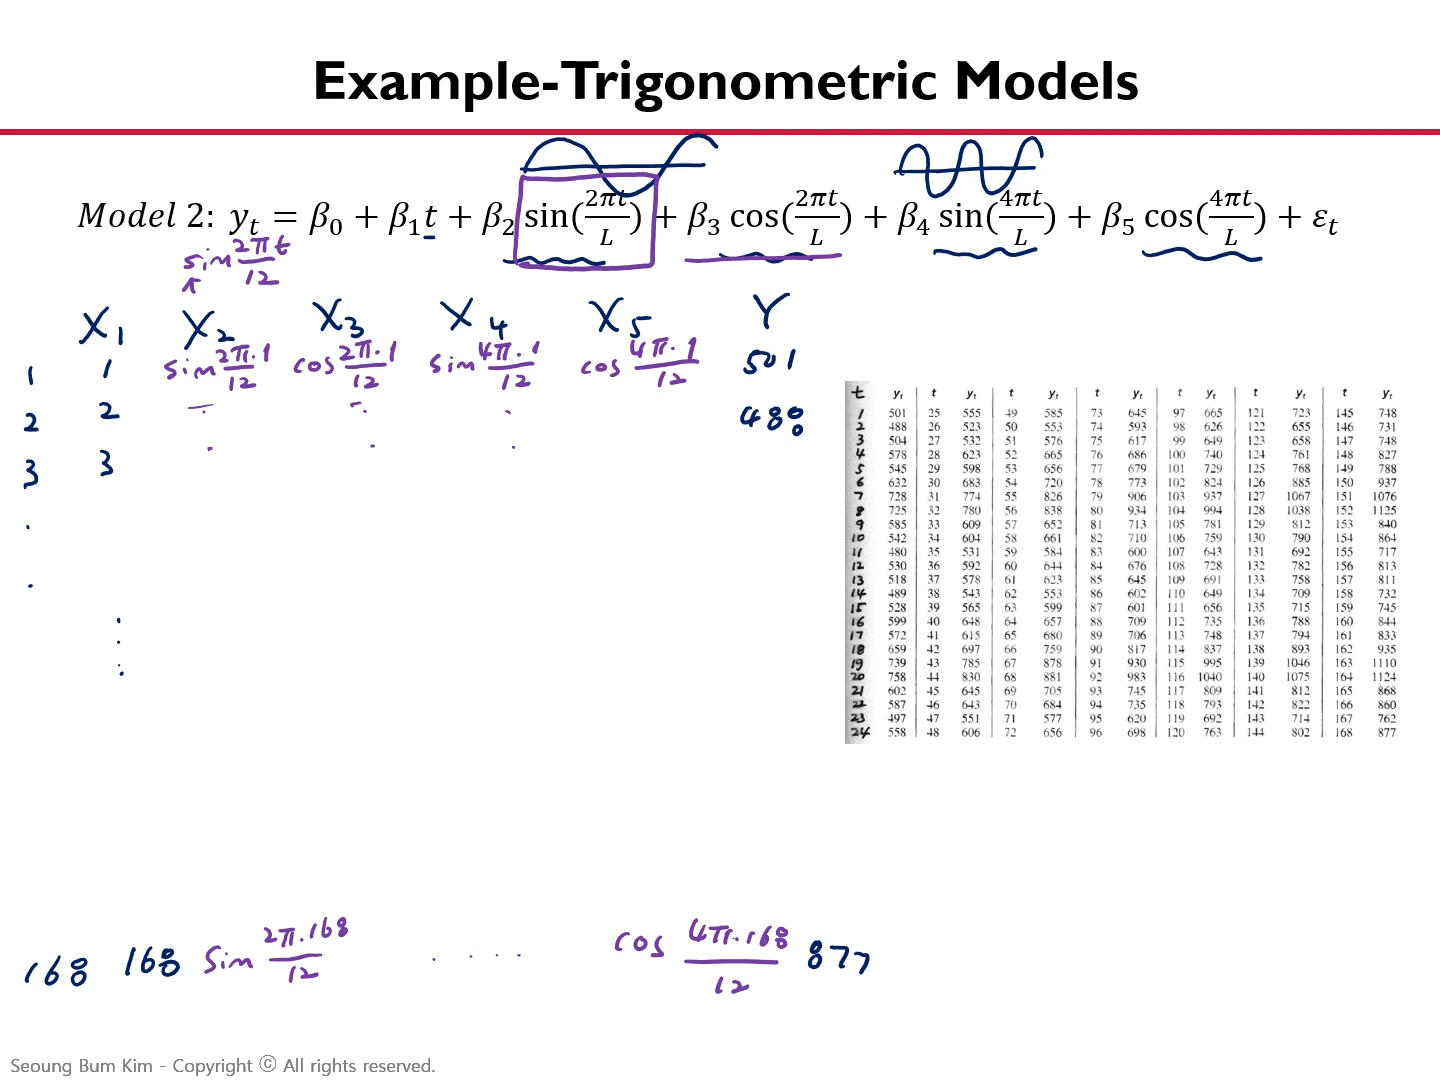
\includegraphics[width=.45\textwidth]{model_2-3}
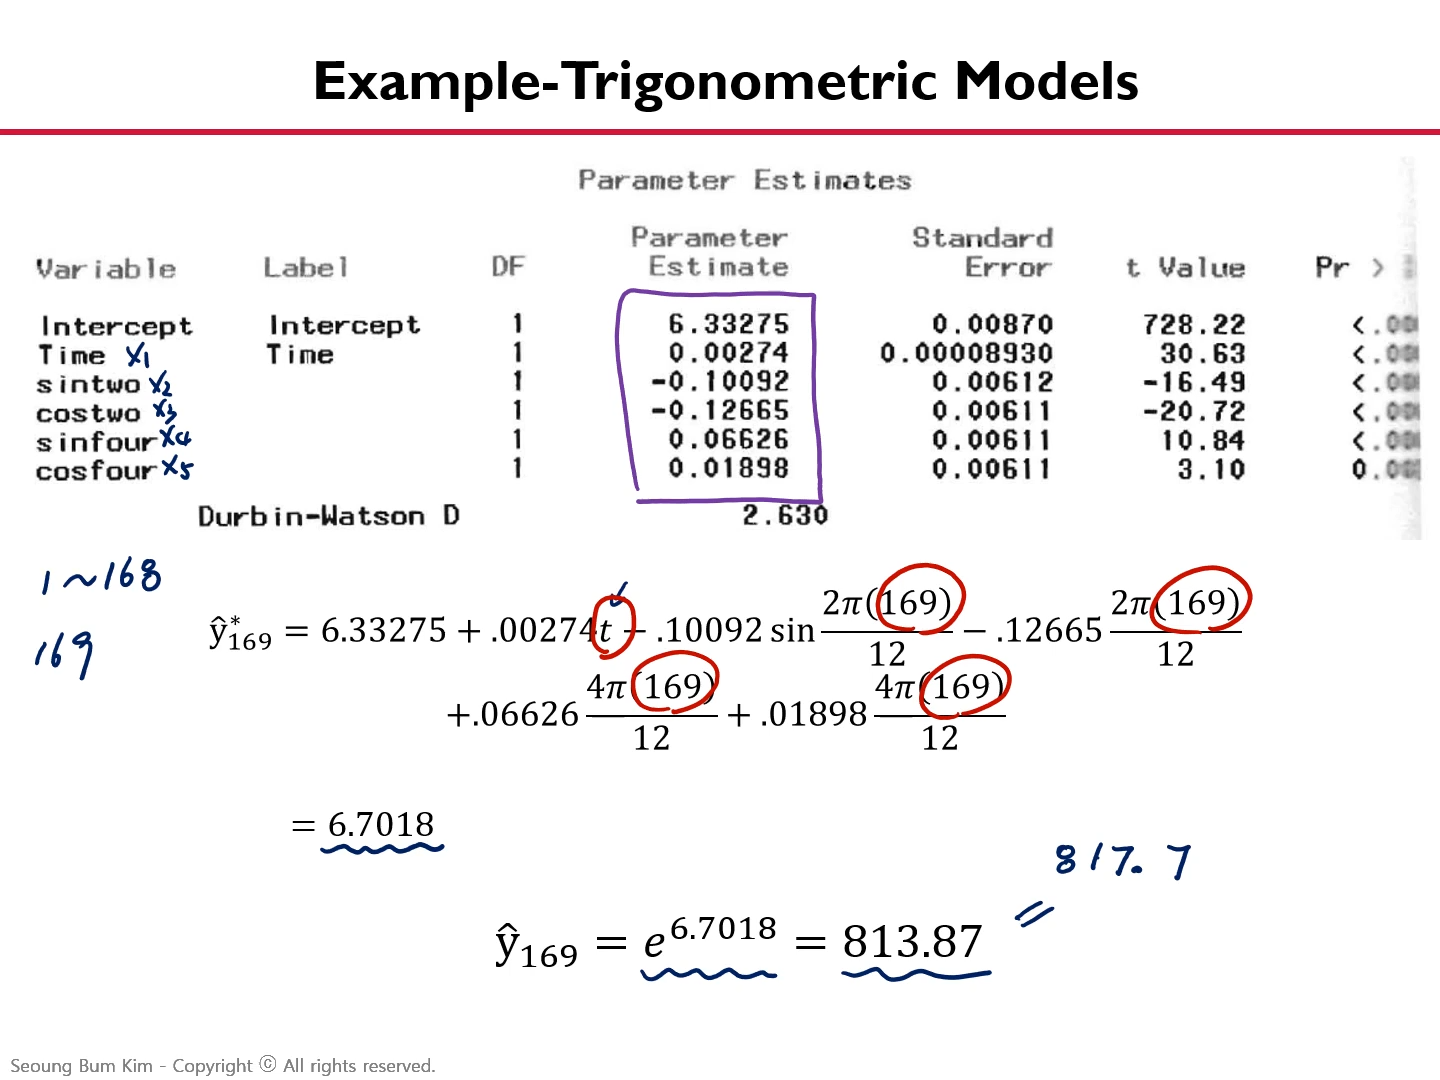
\includegraphics[width=.45\textwidth]{model_2-4}
\end{center}

\(y_t=TR_t+SN_t+\epsilon_t\)에서 \(SN_t\)는 `계절성'을 의미했고, `이것은 일정한 주기를 가지는 패턴'정도로 이해할 수 있었다.
그러니까 \(SN_t\)는 일정한 주기를 가지는 함수, 즉 주기함수이다.
이러한 주기함수를 사인함수와 코사인함수의 일차결합인
\begin{equation}\label{trigonometric_1}
\beta_2\sin\left(\frac{2\pi t}L\right)+\beta_3\sin\left(\frac{2\pi t}L\right)
\end{equation}
로 표현하는 것은 적당해보인다.
식 \eqref{trigonometric_1}은 적당한 실수 \(A=\sqrt{{\beta_2}^2+{\beta_3}^2}>0\), \(B\)에 대하여
\begin{equation}\label{trigonometric_2}
A\cos\left(\frac{2\pi t}L-B\right)
\end{equation}
로 바꿀 수 있으니, 이것은 일반적인 사인함수(코사인함수)를 나타낸다.
그런데 Model 2에서는 주기가 절반인 사인함수와 코사인함수의 일차결합을 더 더해서 표현하고 있다.
이건 아무래도 푸리에 이론과 관련이 있을 것 같다.

푸리에 이론에 따르면, 주기가 \(L\)인 임의의 주기함수 \(g:\mathbb R\to\mathbb R\)는 사인함수와 코사인함수의 급수로 표현할 수 있다.
\[g(t) = \frac{a_0}2+\sum_{k=1}^\infty a_k\sin\left(\frac{2k\pi t}L\right)+b_k\cos\left(\frac{2k\pi t}L\right)\]
그러니까, 함수 \(g_n\)을 (\(n=1,2,\cdots\))
\[g_k(t) = a_k\sin\left(\frac{2n\pi t}L\right)+b_k\cos\left(\frac{2k\pi t}L\right)\]
로 두면 \(\left(g_0(t)=\frac{a_0}2\right)\), Model 1에서 \(SN_t\)는 \(g_0(t)+g_1(t)\)를 의미하고, Model 2에서 \(SN_t\)는 \(g_0(t)+g_1(t)+g_2(t)\)를 의미한다.
\(\sum g_k(t)\)에서 \(n\)을 더 늘려가면, \(\sum g_k(t)\)는 점점 더 \(SN_t\)을 잘 표현할 수 있을 것이다.

다시 돌아와서 말하자면, model 1에서는
\[f_\beta(t)=\beta_0+\beta_1t+\beta_2\sin\left(\frac{2\pi t}L\right)+\beta_3\cos\left(\frac{2\pi t}L\right)\]
로 parametric model을 잡는 것이고, model 2에서는
\[f_\beta(t)=\beta_0+\beta_1t+\beta_2\sin\left(\frac{2\pi t}L\right)+\beta_3\cos\left(\frac{2\pi t}L\right)
+\beta_4\sin\left(\frac{4\pi t}L\right)+\beta_5\cos\left(\frac{4\pi t}L\right)\]
로 두는 것이다.
이 \(f_\beta\)를 가지고 관측치 \eqref{observations}를 MSE \eqref{MSE}에 적용하여 최적화문제를 풀면 \(\hat f\)를 찾을 수 있을 것이다.
네번째 슬라이드에서는 관측치에 로그변환을 적용한 다음 \(SN_t\)을 모델링했으므로 나중에 다시 지수함수를 취해준다.

%%
\section{Growth Curve Models}
\begin{center}
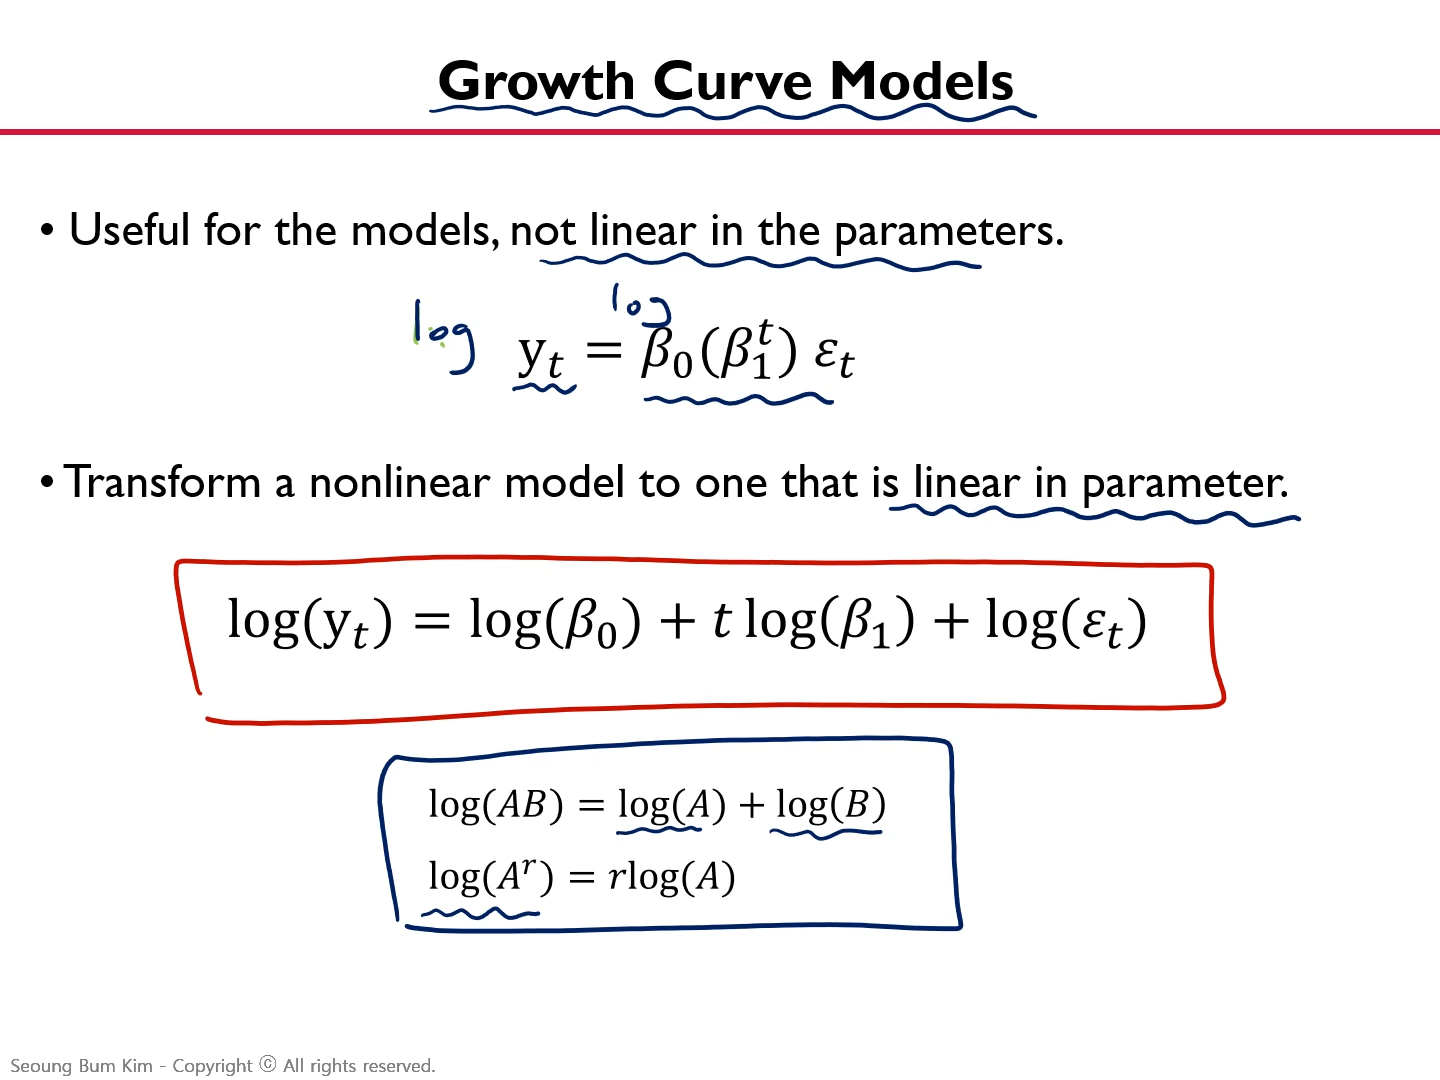
\includegraphics[width=.45\textwidth]{model_3-1}
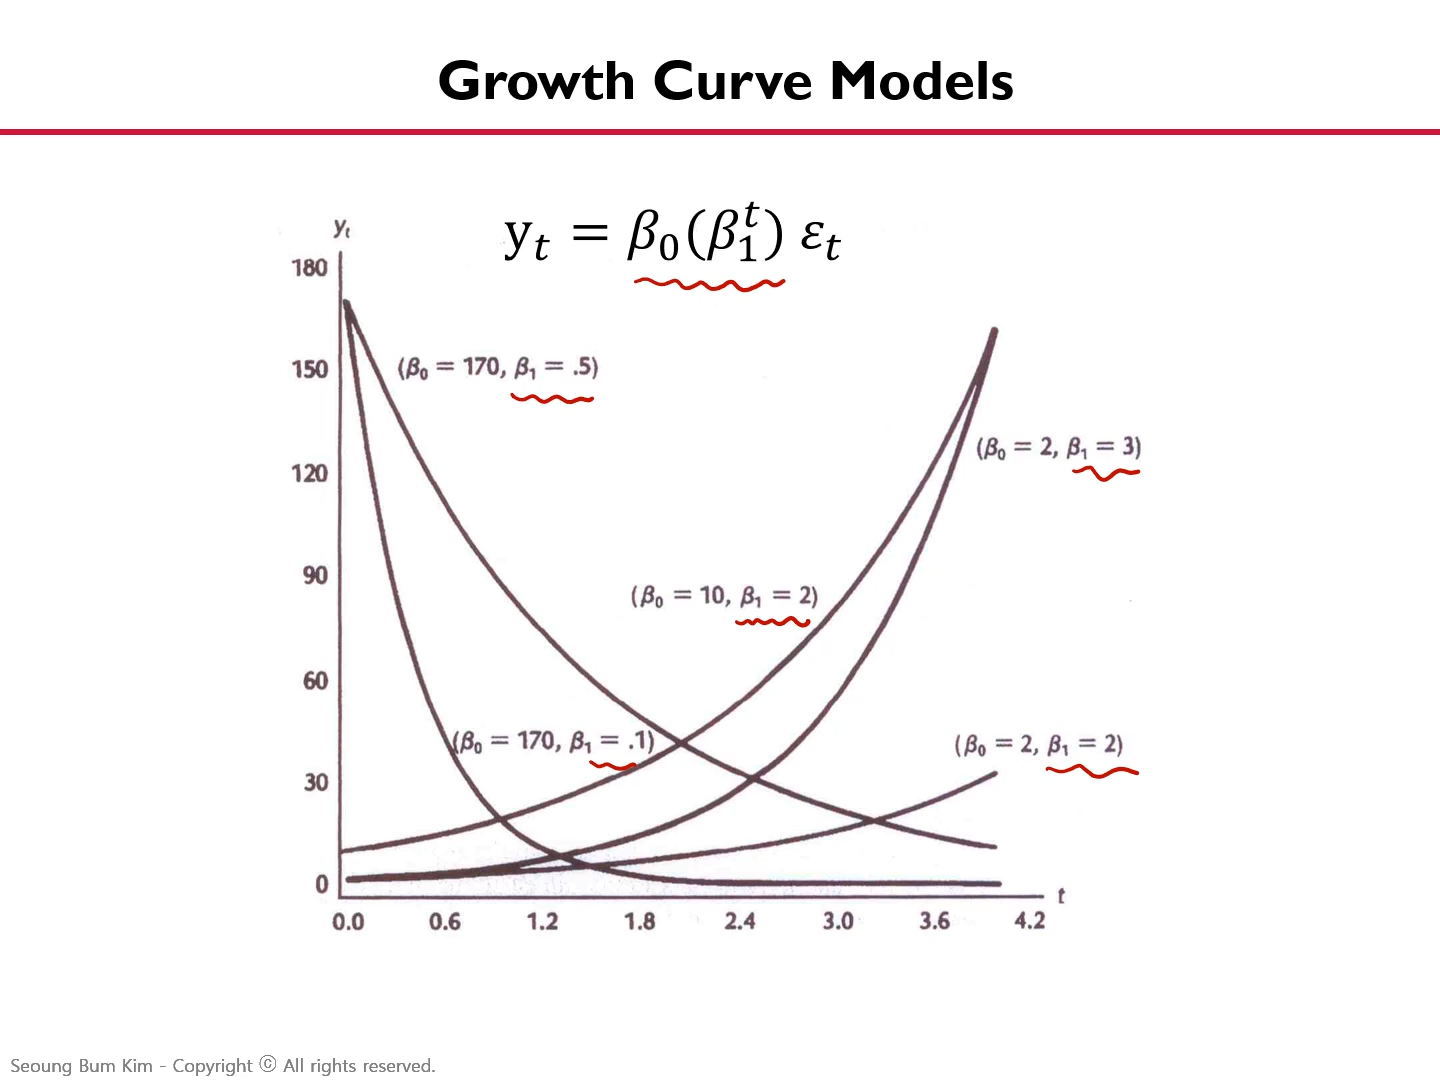
\includegraphics[width=.45\textwidth]{model_3-2}
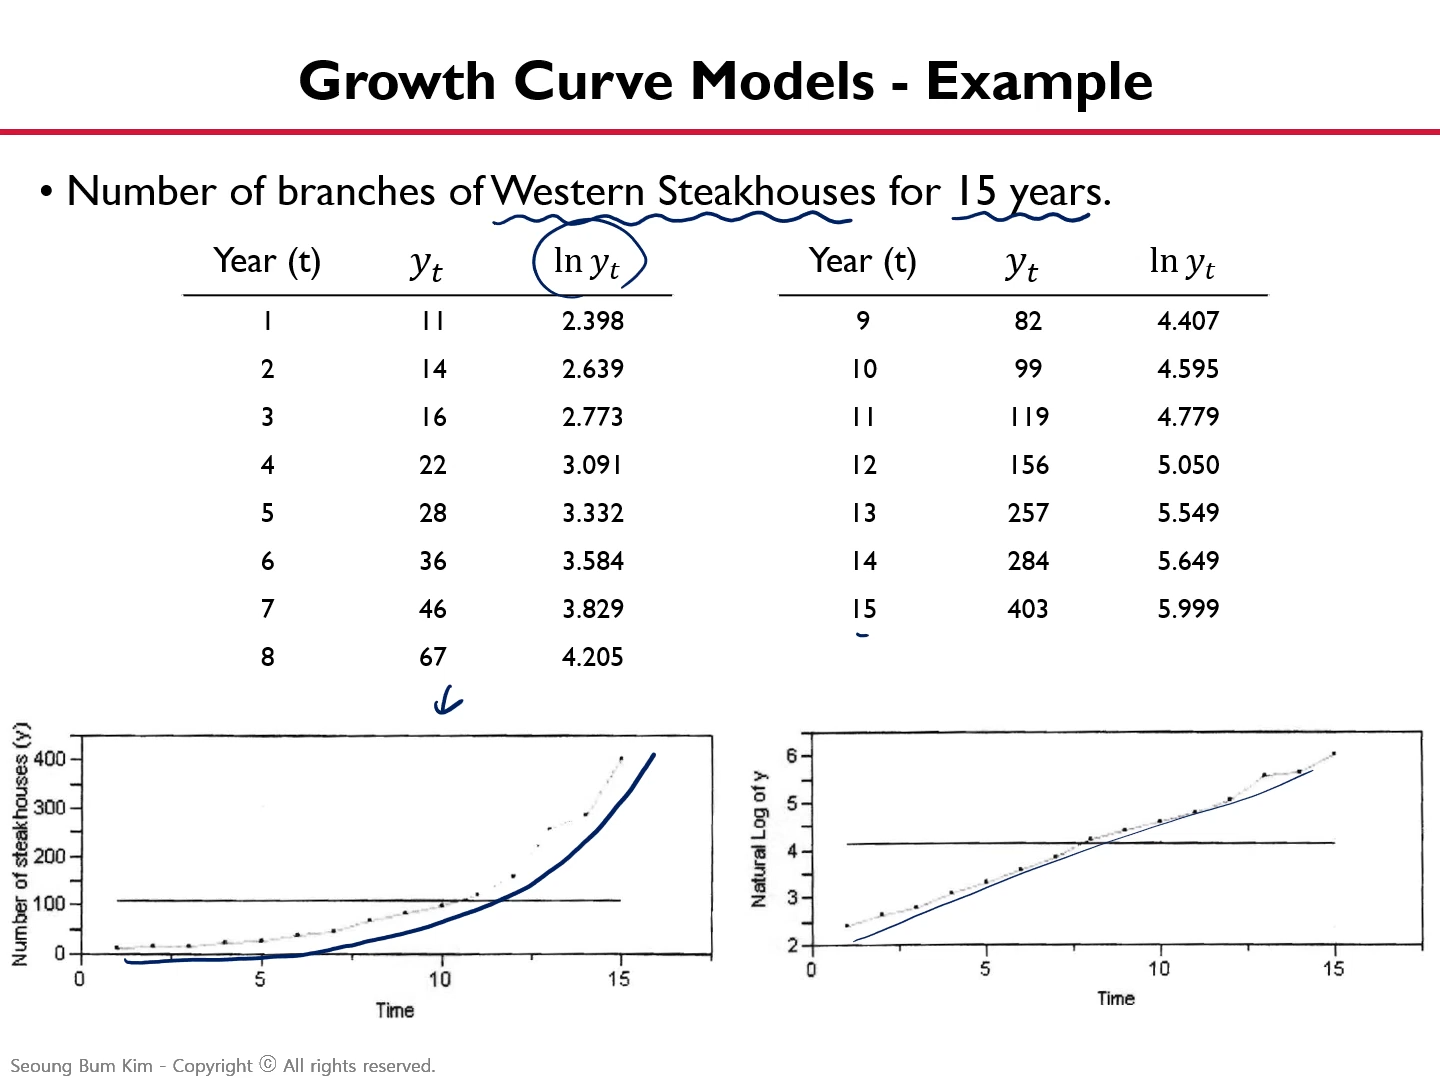
\includegraphics[width=.45\textwidth]{model_3-3}
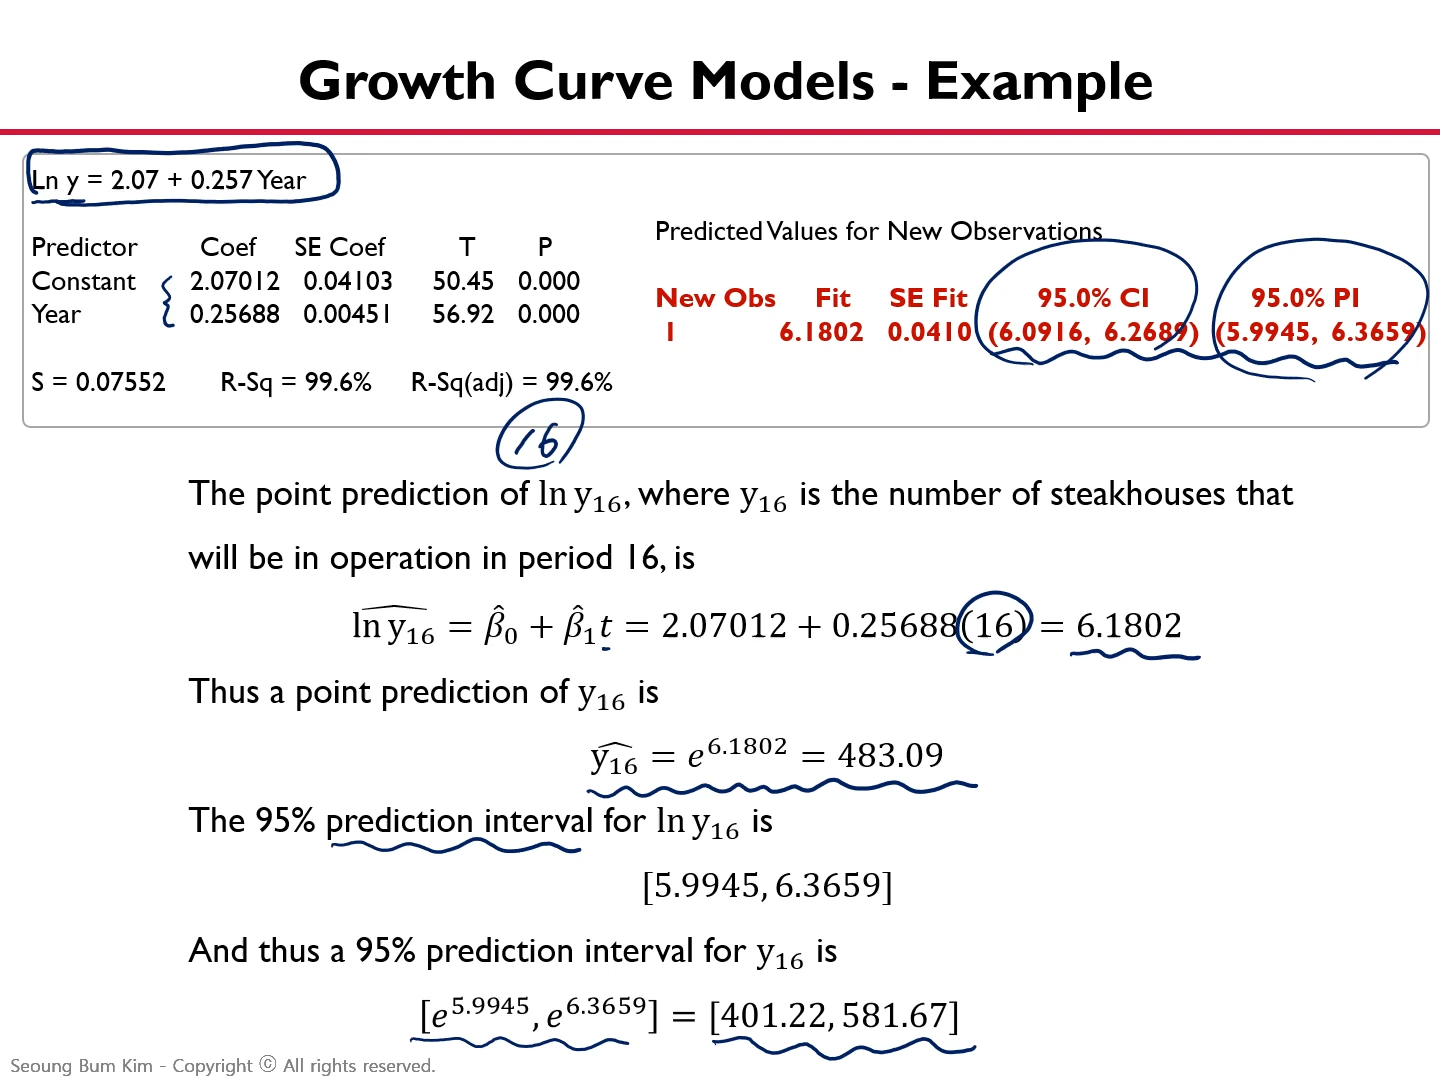
\includegraphics[width=.45\textwidth]{model_3-4}
\end{center}

이번 부분은 왜 있는지 모르겠다.
기존의 모델이 additive한 형식의 모델이었다면, 이건 multipicative model을 설명하려는가본데, 사실 이전 Trigonometric Model에서 로그를 취하여 모델링하는 것을 이미 공부했다.
그리고 지금 위의 캡쳐에 보이는 모델링 방법은 정확히 로그를 취한 linear model과 같아보인다.


%%
\section{First-Order Autoregressive Process}
\begin{center}
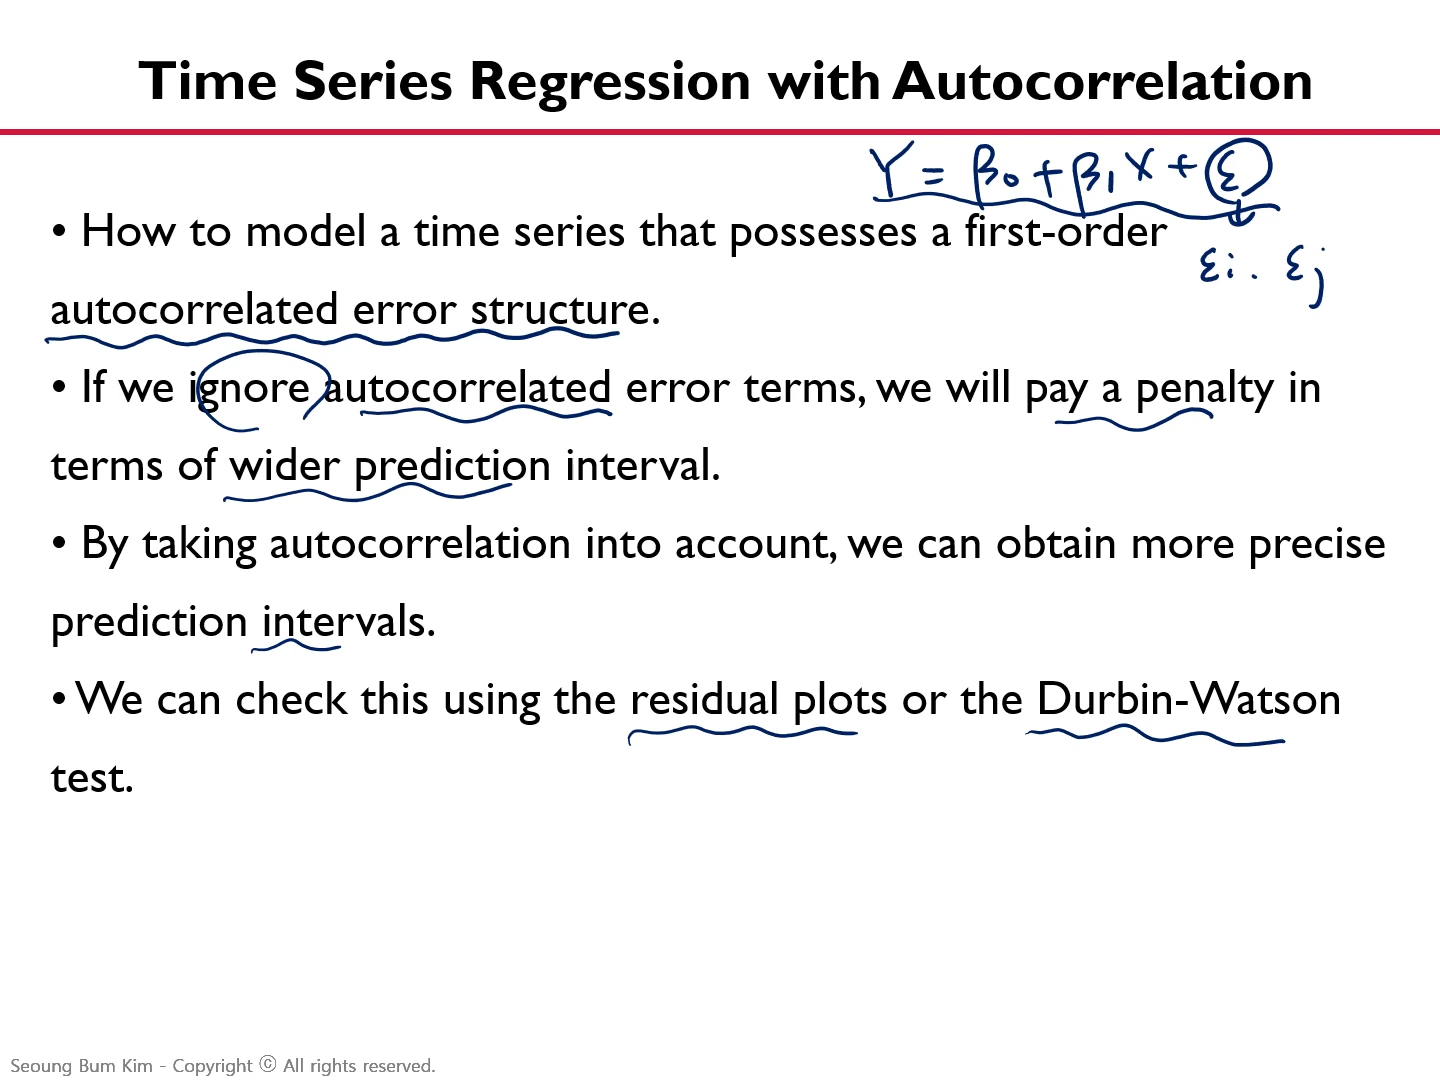
\includegraphics[width=.45\textwidth]{model_4-1}
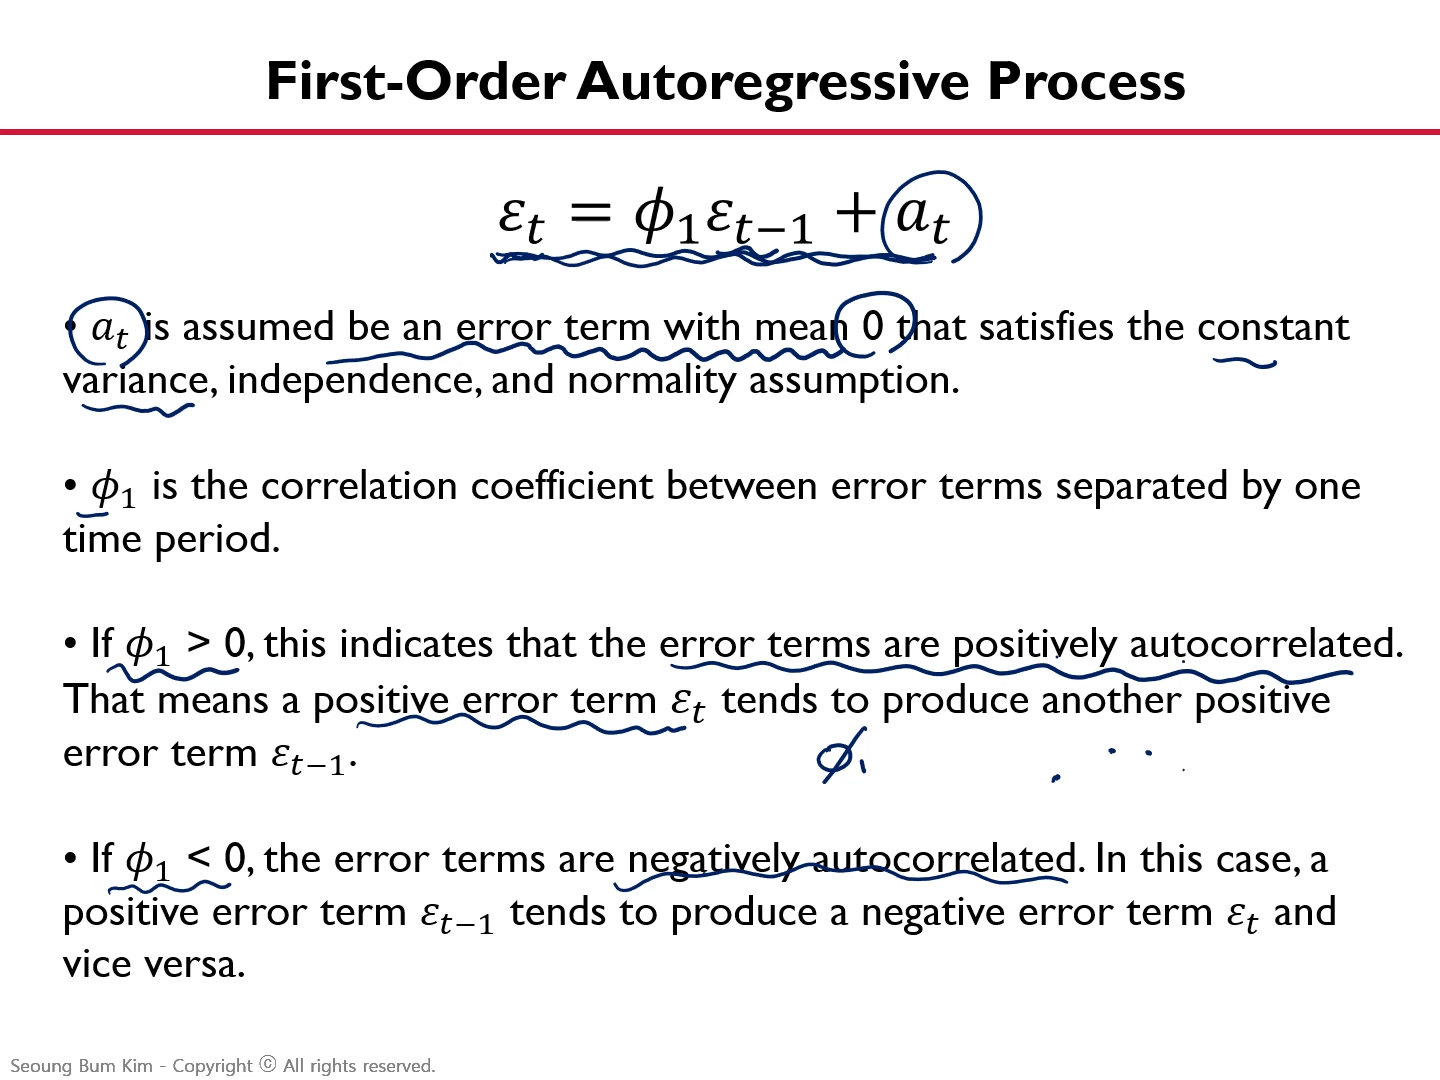
\includegraphics[width=.45\textwidth]{model_4-2}
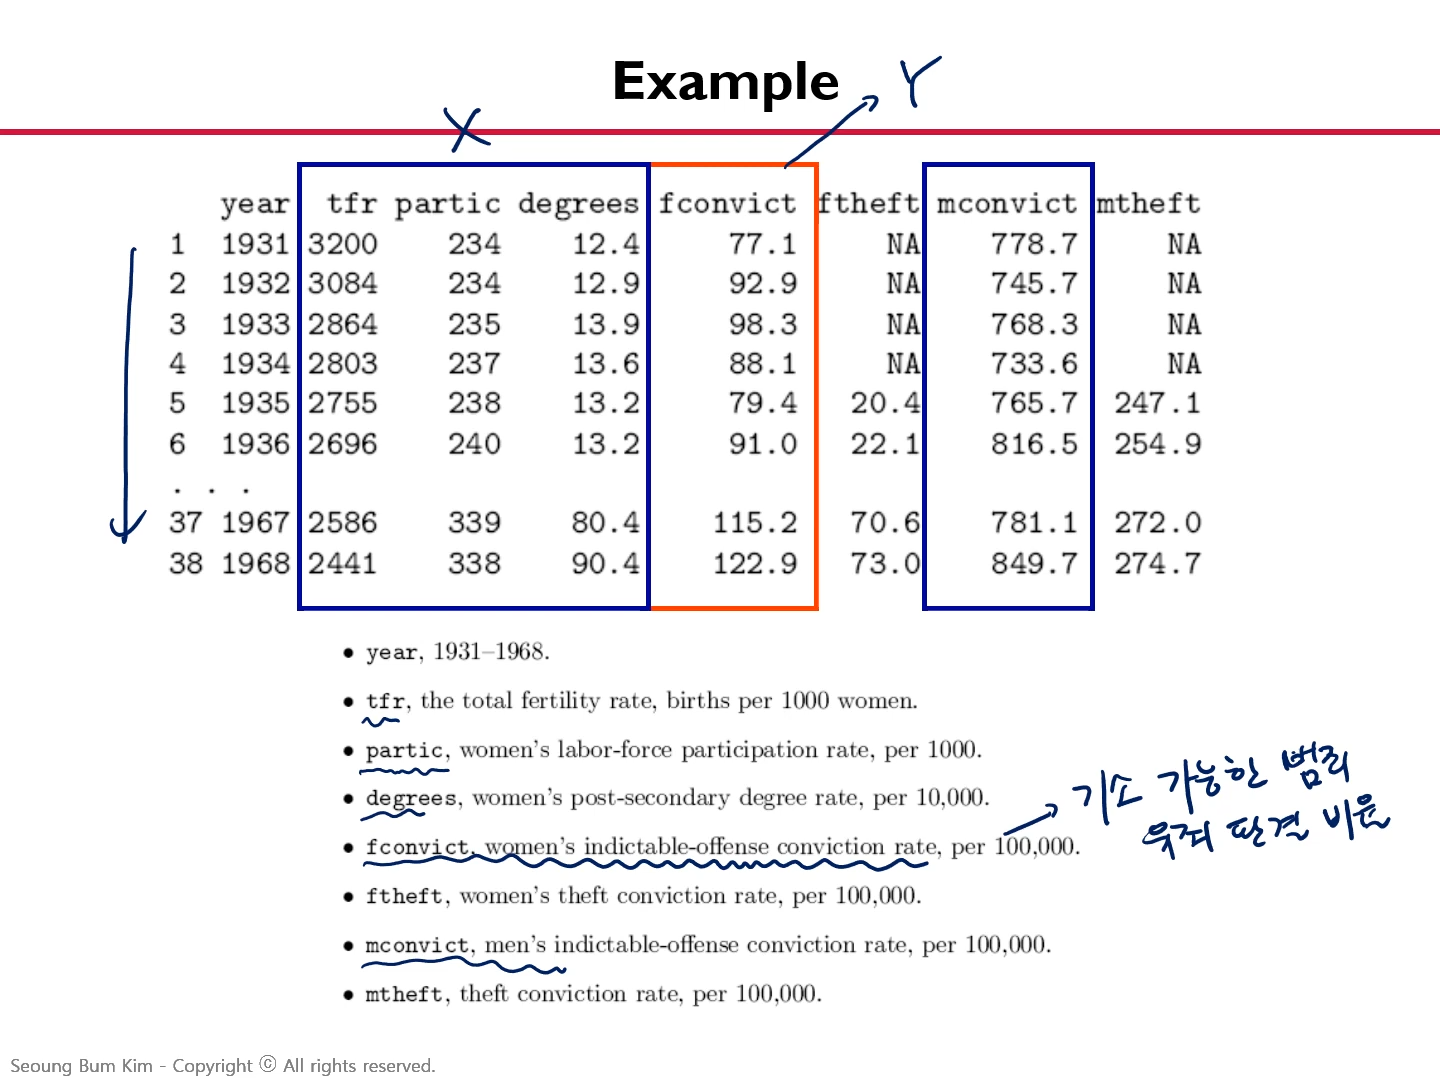
\includegraphics[width=.45\textwidth]{model_4-3}
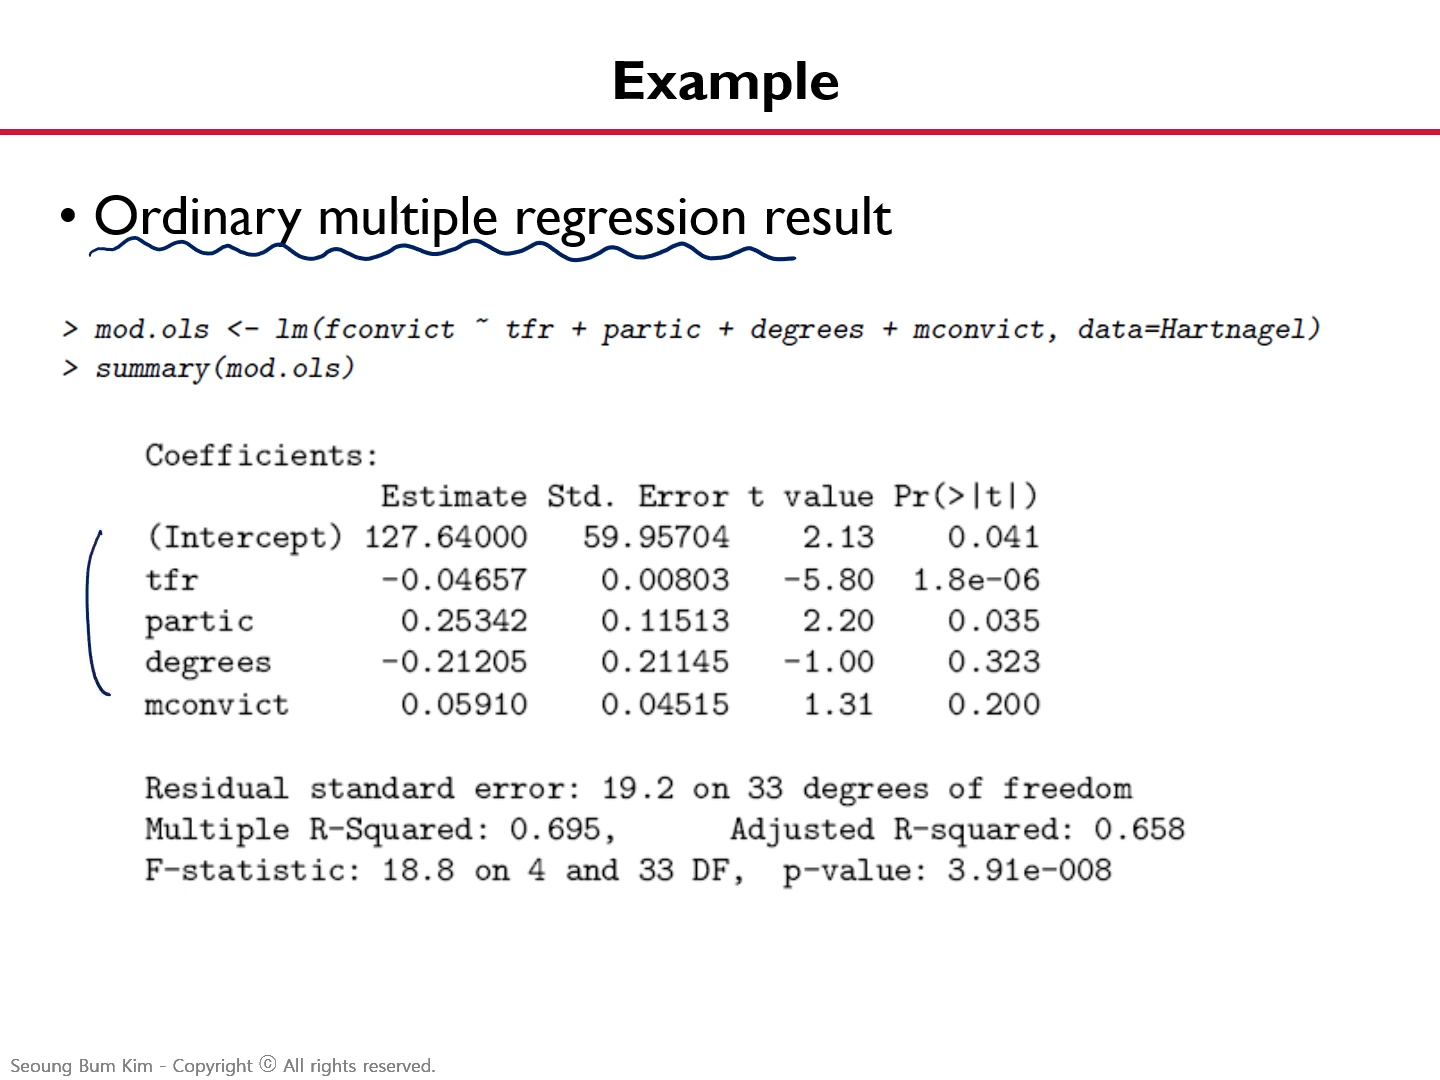
\includegraphics[width=.45\textwidth]{model_4-4}
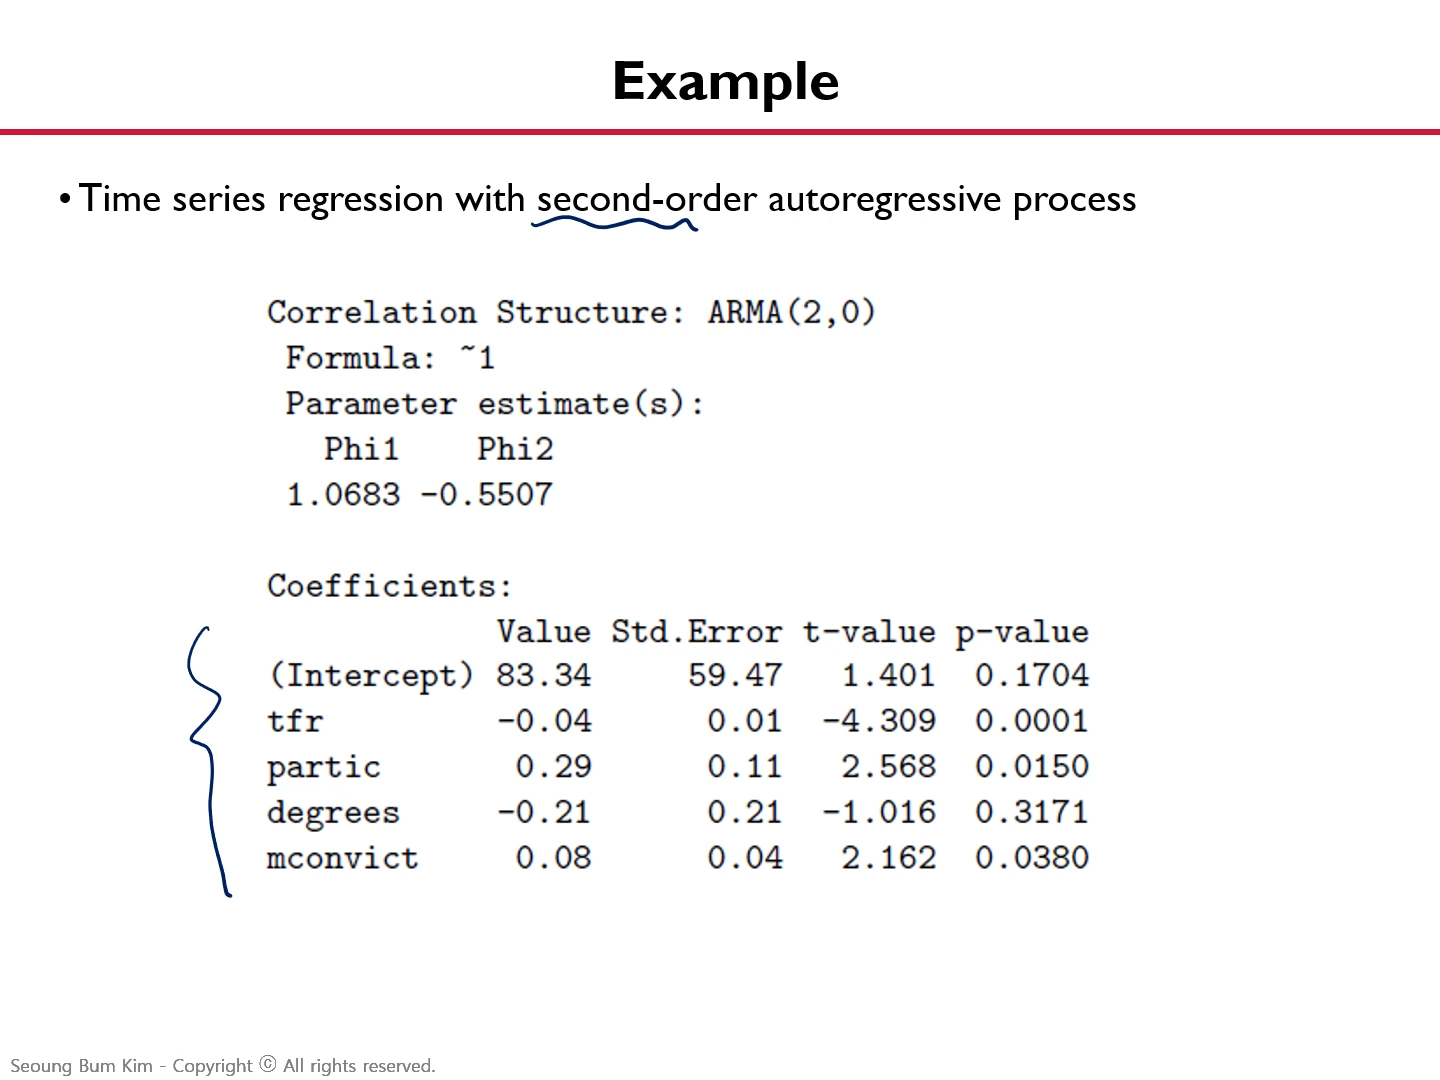
\includegraphics[width=.45\textwidth]{model_4-5}
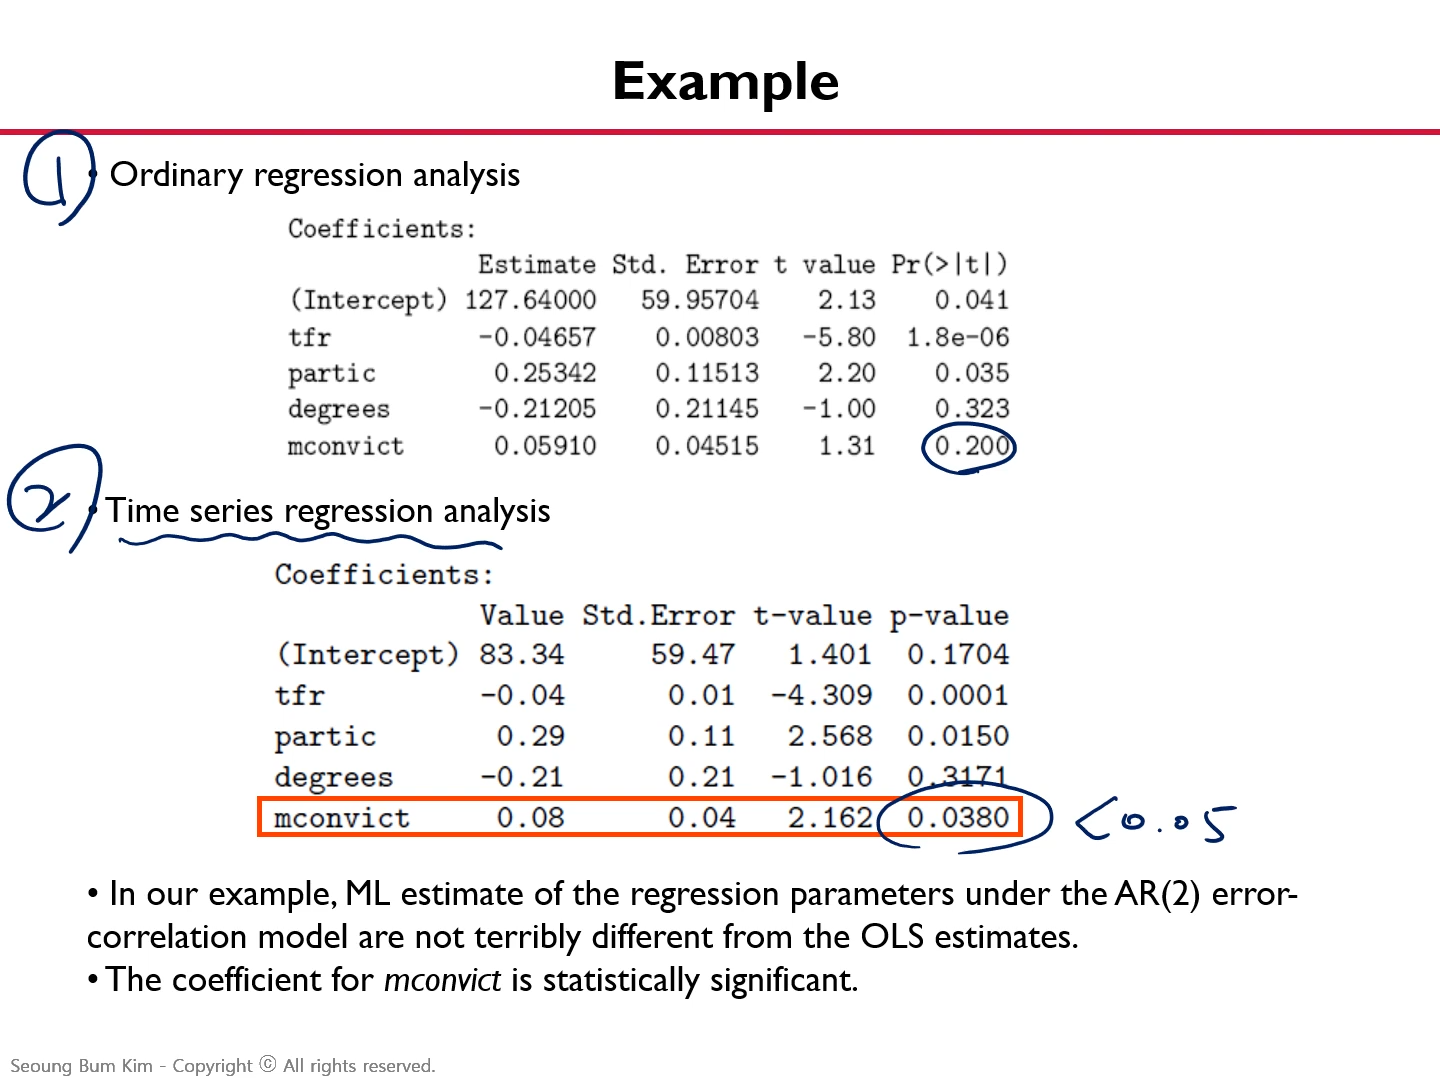
\includegraphics[width=.45\textwidth]{model_4-6}
\end{center}

자세히 읽지 못했다. 아마도, 이전까지는 \(\epsilon_t\)와 \(\epsilon_{t-1}\)이 서로 독립이라는 조건 하에서 논의를 진행시켰던 것 같은데, 여기에서는 두 값이 서로 종속일 수밖에 없으니, \(\epsilon_t\)가 \(\epsilon_{t-1}\)로 표현될 수 있다고 보는 것 같다.
정확하게는 \(\epsilon_t\)가 \(\epsilon_{t-1}\)에 대한 선형함수로 모델링 된다고 보는 것이고, 그 모델링에 대한 error term을 \(a_t\)로 두었다.
\begin{equation}\label{modeling_on_error_term}
\epsilon_t=\phi_1\epsilon_{t-1}+a_t
\end{equation}
\(\phi_1\)은 선형함수에 대한 계수(coefficient) 혹은 기울기이다.

이것을 Durbin-Watson test와 연관지으려면 이전 강의의 노트에 썼던
\begin{gather*}
\epsilon=\{\epsilon_t:t=1,2,\cdots,n\}\\
\epsilon'=\{\epsilon_{t+1}:t=1,2,\cdots,n\}.
\end{gather*}
을 가져오고, 모든 \(t\in\{2,3,\cdots,n\}\)에 대하여 위의 모델링 \eqref{modeling_on_error_term}을 적용시키겠다는 말이다.

강의에서는 Durbin-Watson test에 대해 언급하면서 \(\phi_1>0\)이면 error term들이 positively autocorrelated하다고 말하고, \(\phi_1<0\)이면 negatively autocorrelated하다고 말한다.
하지만 Durbin-Watson test보다는 autocorrelation에 대한 아래 식
\[\rho_1(\epsilon)\rho_1(\epsilon)=\frac{\sum_{t=2}^n\epsilon_t\epsilon_{t+1}}{\sum_{t=2}^n{\epsilon_t}^2}\]
에서 보는 게 더 편할 것 같다.
만약 \(\phi_1>0\)이면, (\(a_t\)의 절댓값이 작을 것이므로) \(\epsilon_t\)와 \(\epsilon_{t-1}\)은 서로 같은 부호인 경우가 많을 것이다.
그러니까 \(\epsilon_t\epsilon_{t-1}\)은 양수가 되는 경우가 많고, 그걸 다 더한 \(\rho_1(\epsilon)\) 값은 양수가 될 것이다.
따라서 \(\epsilon\)은 postively autocorrelated하다.

반대로, 만약 \(\phi_1<0\)이면, \(\epsilon_t\)와 \(\epsilon_{t-1}\)은 서로 다른 부호인 경우가 많을 것이고, \(\epsilon_t\epsilon_{t-1}\)은 음수가 되는 경우가 많다.
따라서 \(\epsilon\)은 negatively autocorrelated하다.




\end{document}